
% mn2esample.tex
%
% v2.1 released 22nd May 2002 (G. Hutton)
%
% The mnsample.tex file has been amended to highlight
% the proper use of LaTeX2e code with the class file
% and using natbib cross-referencing. These changes
% do not reflect the original paper by A. V. Raveendran.
%
% Previous versions of this sample document were
% compatible with the LaTeX 2.09 style file mn.sty
% v1.2 released 5th September 1994 (M. Reed)
% v1.1 released 18th July 1994
% v1.0 released 28th January 1994


\documentclass[useAMS,usenatbib]{mn2e}
\usepackage{graphicx}
\usepackage{float}
\usepackage{wasysym}
%\usepackage{stmaryrd}
\usepackage{txfonts}
\usepackage{natbib}
\usepackage{color}
\usepackage{colortbl}
\usepackage{multirow}

% Journal Definitions
\def   \aj {{\rm {AJ}}}
\def   \araa {{\rm {ARA\&A}}}
\def   \apj {{\rm {ApJ}}}
\def   \icarus {{\rm {Icarus}}}
\def   \apjs {{\rm {ApJS}}}
\def   \apss {{\rm {Ap\&SS}}}
\def   \aap {{\rm {A\&A}}}
\def   \aapr {{\rm {A\&AR}}}
\def   \aaps {{\rm {A\&AS}}}
\def   \baas {{\rm {BAAS}}}
\def   \memras {{\rm {MmRAS}}}
\def   \mnras {{\rm {MNRAS}}}
\def   \prl {{\rm {Phys. Rev. Lett.}}}
\def   \jqsrt {{\rm {Journal of Quantitative Spectroscopy and Radiative Transfer}}}
\def   \apjl{\rm {ApJL}}
\def   \nat{\rm {Nat.}}
\def   \pasj{\rm {PASJ}}


% If your system does not have the AMS fonts version 2.0 installed, then
% remove the useAMS option.
%
% useAMS allows you to obtain upright Greek characters.
% e.g. \umu, \upi etc.  See the section on "Upright Greek characters" in
% this guide for further information.
%
% If you are using AMS 2.0 fonts, bold math letters/symbols are available
% at a larger range of sizes for NFSS release 1 and 2 (using \boldmath or
% preferably \bmath).
%
% The usenatbib command allows the use of Patrick Daly's natbib.sty for
% cross-referencing.
%
% If you wish to typeset the paper in Times font (if you do not have the
% PostScript Type 1 Computer Modern fonts you will need to do this to get
% smoother fonts in a PDF file) then uncomment the next line
% \usepackage{Times}

%%%%% AUTHORS - PLACE YOUR OWN MACROS HERE %%%%%


%%%%%%%%%%%%%%%%%%%%%%%%%%%%%%%%%%%%%%%%%%%%%%%%

\title[Young protoplanetary discs]{Simulated Observations of Young Gravitationally Unstable Protoplanetary Discs}
%%authors arent splitting over 2 lines so rawlings is pushed off the edge
%\author[Tom Douglas, Paola Caselli, Et al.]{Tom Douglas$^{1}$\thanks{E-mail:
%pytd@leeds.ac.uk}, Paola Caselli$^{1}$, Aaron Boley$^{2}$, Richard Durisen$^{3}$, Tom Hartquist$^{1}$, %John Ilee$^{1}$, Jonathon Rawlings$^{4}$ \\
%$^{1}$School of Physics and Astronomy, University of Leeds, Leeds LS2 9JT, UK \\
%$^{2}$Department of Astronomy, University of Florida, 211 Bryant Space Center, PO Box 112055, USA\\
%$^{3}$Department of Astronomy, Indiana University, 727 East 3rd Street, Swain West 319, Bloomington, IN %47405, USA\\
%%$^{4}$Department of Physics & Astronomy, University College London, London WC1E 6BT, UK\\
%}

\author[T.~A.~Douglas et al.]
{\parbox{\textwidth}{T. A. Douglas$^{1}$\thanks{E-mail: \texttt{pytd@leeds.ac.uk}},
P. Caselli$^{1}$,
J. D. Ilee$^{1}$,
A. C. Boley$^{2}$,
T. W. Hartquist$^{1}$,
R. H. Durisen$^{3}$, and
J. M. C. Rawlings$^{4}$\\
\vspace{0.1cm}\\
{\small{\it$^{1}$School of Physics and Astronomy, University of Leeds, Leeds LS2 9JT, UK,}} \\
{\small{\it$^{2}$Department of Astronomy, University of Florida, 211 Bryant Space Center, PO Box 112055, USA,}}\\
{\small{\it$^{3}$Department of Astronomy, Indiana University, 727 East 3rd Street, Swain West 319, Bloomington, IN 47405, USA,}}\\
{\small{\it$^{4}$Department of Physics \& Astronomy, University College London, London WC1E 6BT, UK}}\\}}


%{\parbox{\textwidth}{
%$^{1}$School of Physics and Astronomy, University of Leeds, Leeds LS2 9JT, UK \\
%$^{2}$Department of Astronomy, University of Florida, 211 Bryant Space Center, PO Box 112055, USA\\
%$^{3}$Department of Astronomy, Indiana University, 727 East 3rd Street, Swain West 319, Bloomington, IN %47405, USA\\
%$^{4}$Department of Physics & Astronomy, University College London, London WC1E 6BT, UK\\
%}}



\begin{document}

\date{Jan 2013}

\pagerange{\pageref{firstpage}--\pageref{lastpage}} \pubyear{2002}

\maketitle

\label{firstpage}

\begin{abstract}
The formation and earliest stages of protoplanetary discs are still lacking observational constraints. ALMA will soon revolutionize this field, therefore it is important to provide predictions and help the interpretation of future high sensitivity and high angular resolution observations. Here we present simulated ALMA observations based on radiative transfer modelling of a relatively massive (0.39 M$_{\odot}$) self-gravitating disc embedded in a 10\,M$_{\odot}$ dense core, with structure similar to the pre-stellar core L1544. We focus on simple species and conclude that  C$^{17}$O 3$\rightarrow$2, HCO$^+$ 3$\rightarrow$2, OCS 26$\rightarrow$25 and H$_2$CO 4$_{04}\rightarrow$3$_{03}$ lines together allow for measurements of the disc structure and kinematics at all scales. 
\end{abstract}

\begin{keywords}
Stars: Circumstellar Matter -- infrared; Stars: Formation -- infrared; Planetary Systems: Protoplanetary Discs.
\end{keywords}

\section{Introduction}

The formation and early evolution of protoplanetary discs around solar-type and low-mass protostars has little observational support, despite of the fast growing list of theoretical models on the dynamical evolution of star forming dense cores (e.g. \citealt{Krasnopolsky2011,Machida2011,Braiding2012,Joos2013}). The reason for this is that young protostars are surrounded by thick envelopes and power energetic outflows. Thus, observations of the young discs, predicted to have sizes of about 100\,au and masses as large as 10\% the original core mass (e.g. \citealt{Joos2012,Hayfield2011,Machida2011}), are challenging. The use of sensitive interferometers is needed to achieve high angular resolution and spatially/spectrally disentangle the various disc, envelope and outflow components as well to filter out the extended emission tracing envelope material. \smallskip

After the pioneer work of, e.g., \citet{Chandler1995,Brown2000,Looney2000}, recent interferometric observations have discovered compact embedded discs in a sample of Class 0 sources \citep{Andre1999}, finding masses between 0.4 and  $>$1 M$_{\odot}$ \citep{Jorgensen2007,Jorgensen2009,Enoch2011}. A 130\,au disc was discovered toward a Class 0 source in Perseus, using the Jansky Very Large Array (JVLA) to observe NH$_3$ \citep{Choi2007}. \citet{Pineda2012} observed methyl formate (HCOOCH$_3$) with the Atacama Large Millimetre/sub-millimetre Array (ALMA) and found evidence of rotation toward one of the proto-binary Class 0 sources embedded in IRAS 16293-2422. These observations are consistent with an almost edge-on disc. \citet{Persson2012} observed H$_2^{18}$O with ALMA toward the same source and found evidence of relatively large ($\ga$100\,K) excitation temperatures, as well as a HDO/H$_2$O abundance ratio close to that measured on Earth's oceans and Jupiter-family comets \citep{Hartogh2012}. \citet{Zapata2013} used ALMA to observe a disc of size $\sim$50$\,$au in the other Class 0 source in IRAS 16293-2422 and detected infall towards this disc as inverse P-Cygni profiles in HCN and CH$_3$OH. When ALMA is completed, it will be finally possible to spatially resolve these young discs and, for the first time, put stringent constraints on the theoretical models mentioned previously. As full-operational ALMA is fast approaching, it is important to provide observational predictions based on dynamical models of young protoplanetary discs. \smallskip 

Simulated observations of gravitationally unstable discs have already been performed to study the continuum emission, measure the structure and investigate possible fragmentation \citep{Cossins2010,Ruge2013}. Molecular line emission from massive discs has been simulated by \citet{Krumholz2007}, assuming local thermodynamic equilibrium (LTE). In this paper, we focus on the self-gravitating discs of \citet{Boley2008}, where episodic heating induced by spiral shocks is present. This may be a good representation of the earliest phases of protoplanetary discs and an alternative to the young ``static'' discs studied by, e.g., \citet{Visser2009,Visser2011}. As shown by \citet{Ilee2011}, hereafter I2011, the spiral shocks cause desorption of volatiles from dust icy mantles and trigger gas-phase chemical reactions with activation energies, too high to occur at lower temperatures. These processes produce clear chemical signatures of the disc dynamics. With the use of non-LTE 3D radiative transfer modelling, we perform simulated ALMA observations of the disc studied by I2011 and identify the best tracers of the physical structure of self-gravitating discs. The physical, chemical and radiative transfer models are described in Sect.\,\ref{sec:description_model}. Radiative transfer results are in Sect.\,\ref{sec:model_results}, while ALMA simulated observations are in Sect.\,\ref{sec:alma_predictions}. Discussions and conclusions can be found in Sect.\,\ref{sec:discussion}. 

\section{Description of the Model} \label{sec:description_model}

\subsection{Physical structure} \label{subsec:physical_structure}

To appropriately describe the environment within which a young protoplanetary disc is embedded, we combine the disc model from I2011 with a model of a dense core with characteristics similar to the well-studied pre-stellar core L1544 (\citealt{Keto2010}, hereafter KC2010). Although L1544 does not appear to contain a central protostar and disc itself, other similar dense cores such as L1521F contain a central object which appears to be a low mass protostar and disc \citep{Bourke2006} whilest having around half the mass of L1544. The KC2010 model follows the dynamical, chemical and thermal evolution of a contracting Bonnor-Ebert sphere \citep{Bonnor1956,Ebert1957} with total mass of 10\,M$_{\odot}$, until it reaches the density, temperature and velocity profiles which best match observations. The pre-stellar core model adopted here contains slight modifications due to the inclusion of oxygen cooling in the outer regions of the cloud, where CO is mostly photodissociated \citep{Caselli2012}. Figure \ref{fig:l1544_model} shows the physical parameters of the core model. \smallskip

\begin{figure}
 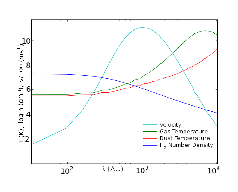
\includegraphics[width=84mm]{Figures/model/L1544model_used_legend_small.eps}
 \caption{The spherically symmetric model of the pre-stellar core L1544 used as the envelope of the young protoplanetary disc in the hybrid model. Showing gas (green) and dust (red) temperature in kelvin, log number density (blue) in cm$^{-3}$ and inward velocity / 10 (cyan) in m$\,$s$^{-1}$. Adapted from KC2010 and Keto et al. (2013, in preparation).}
 \label{fig:l1544_model}
\end{figure}

\begin{figure}
 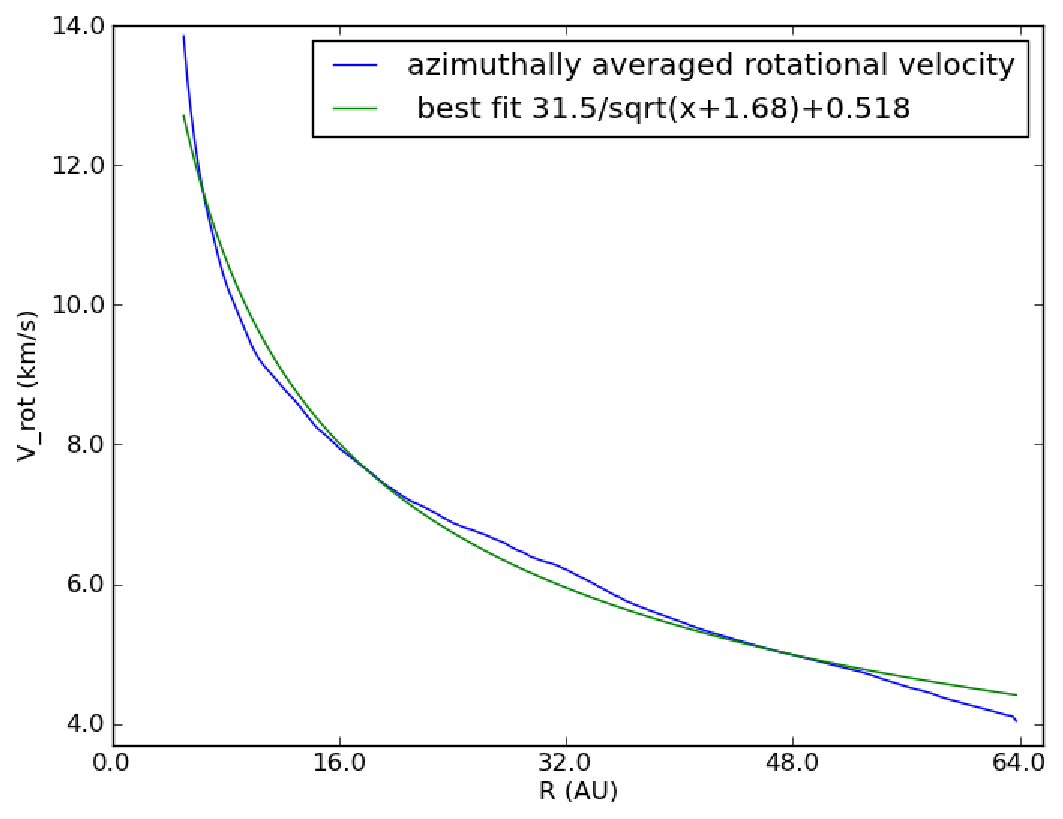
\includegraphics[width=84mm]{Figures/model/rotational_velocities.eps}
 \caption{Azimuthaly averaged rotational velocity in the disc mid-plane. The best fit curve follows the equation $\frac{31.5}{\sqrt{x+1.68}}+0.518$ .}
 \label{velocity}
\end{figure}

\begin{figure*}
 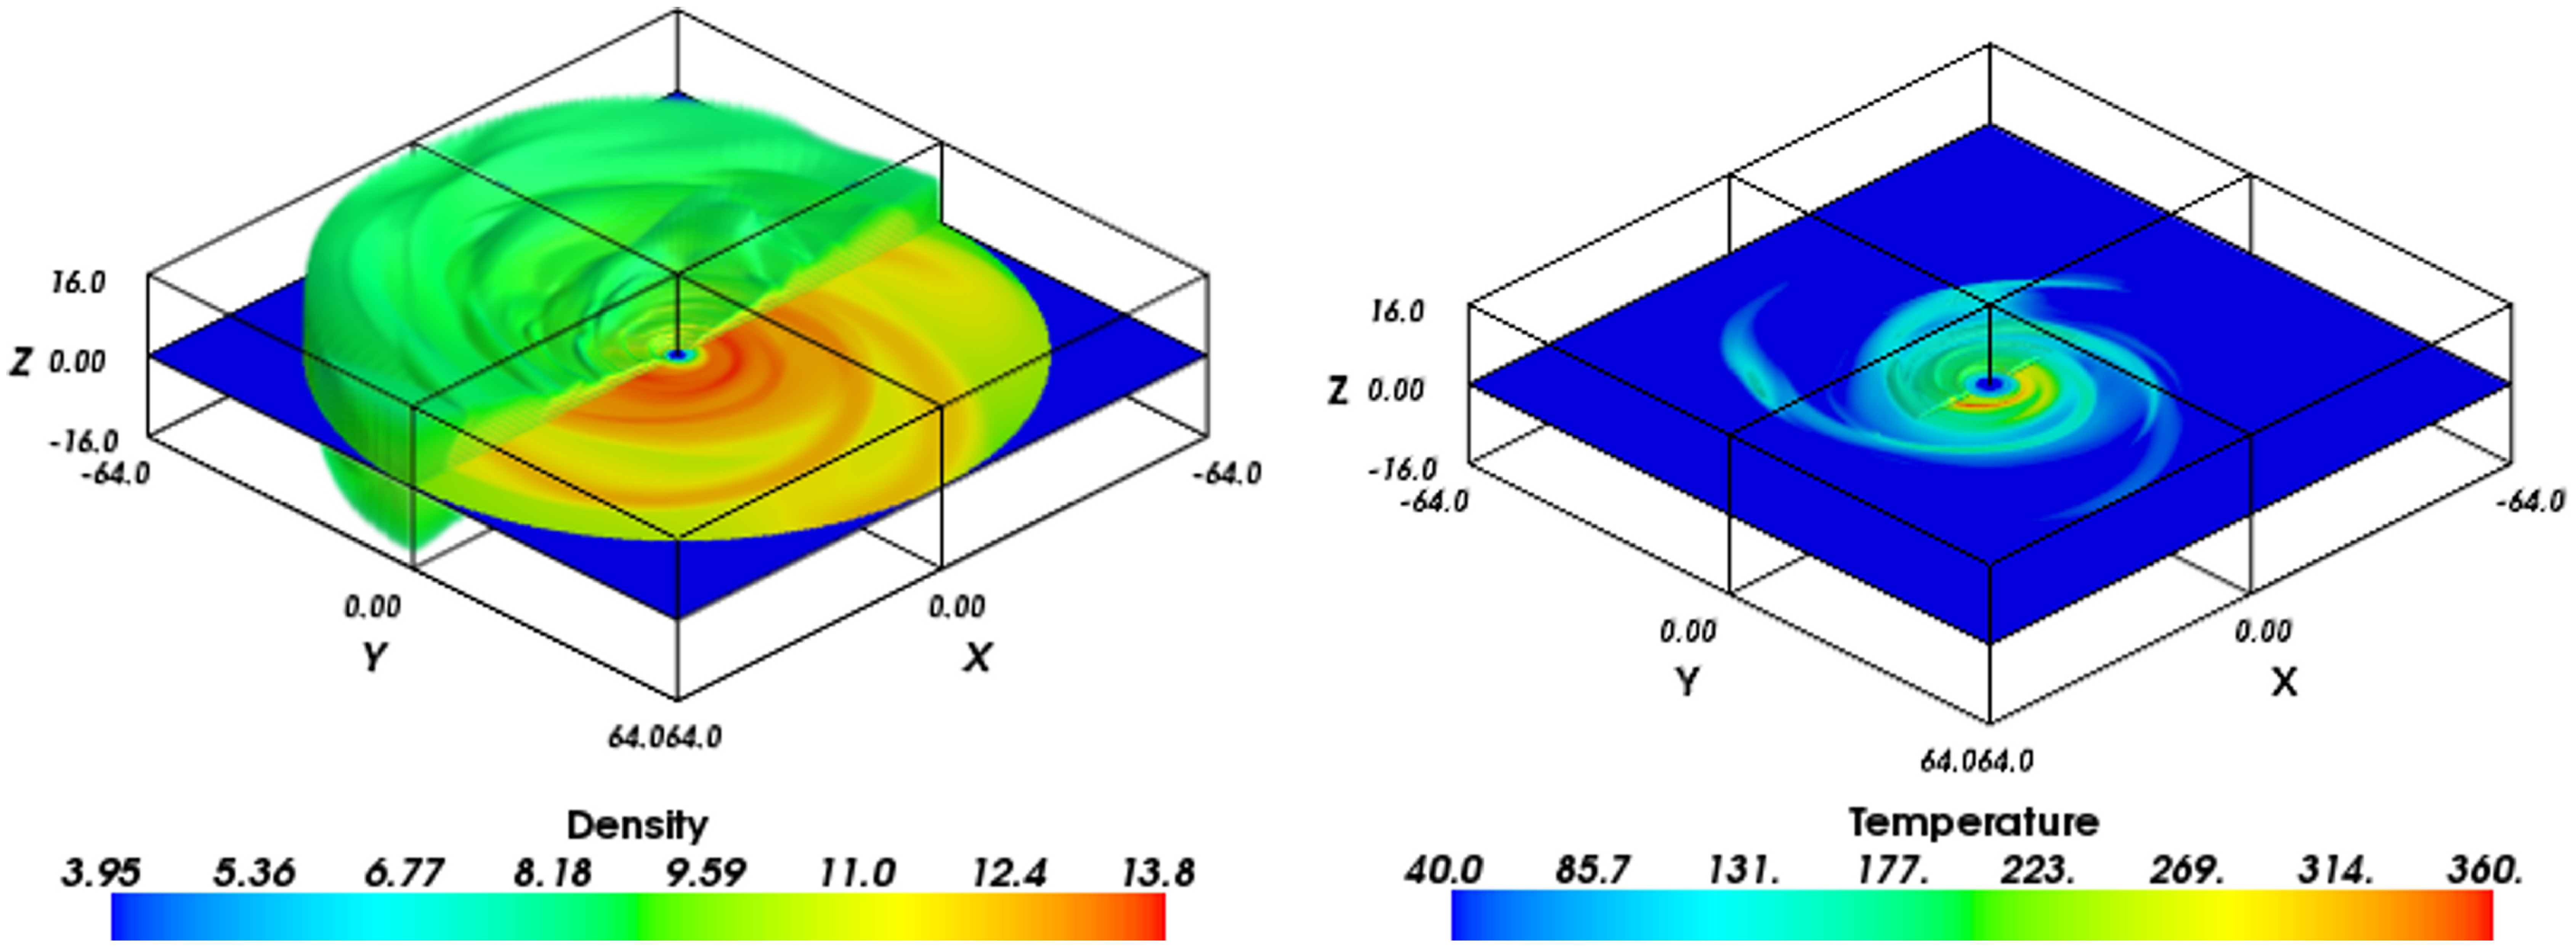
\includegraphics[width=168mm]{Figures/model/rhoT6.eps}
 \caption{{\bf Left:} A 3D plot of log number density (cm$^{-3}$) showing the spiral structure in the xy plane and scale height of the disc. {\bf Right:} The 3D temperature (K) structure of the disc; regions cooler than 40$\,$K are not shown in 3D, highlighting the narrow central region containing hot material.}
 \label{rhoT} 
\end{figure*}

\begin{figure*}
 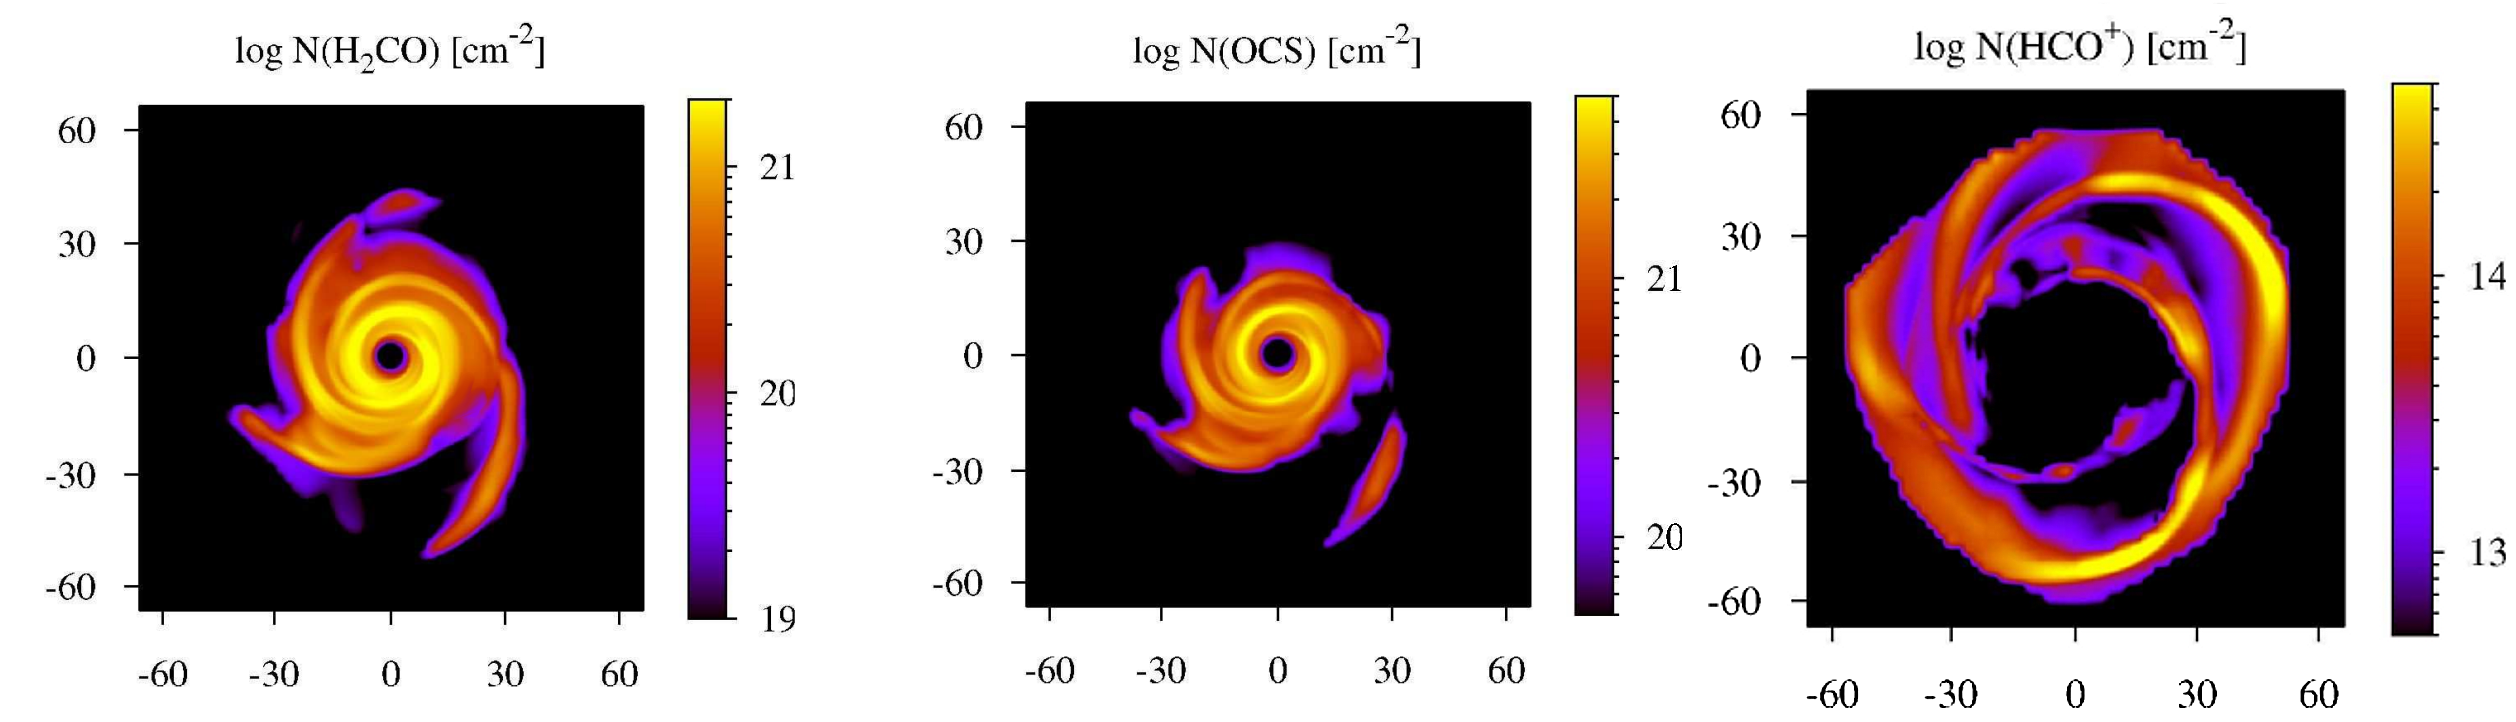
\includegraphics[width=168mm]{Figures/model/columnDensities2.eps}
 \caption{Column densities of OCS, H$_2$CO,HCO$^+$ and CO used in the disc model. Figure adapted from I2011.}
 \label{Chemistry} 
\end{figure*}




The pre-stellar core structure is maintained down to a radius of 80\,au, within which the model of the young protoplanetary disc is used. The disc structure used is from the same hydrodynamics simulation described in I2011, which is a 1$\,$M$_\odot$ protostar surrounded by a 0.39$\,$M$_\odot$ disc. The system is envisaged to be at a very early stage of evolution and embedded in an envelope.  The still growing protostar will eventually become an A star through accretion of most of the disc's mass. The hydrodynamics simulation is run with a proper equation of state for molecular hydrogen \citet{Boley2007}.  The star is allowed to move freely in response to disc torques, and radiative cooling is included \citet{Boley2009}. The self-gravitating disc exhibits prominent spiral structure, with H2 number densities in the disc ranging from 10$^4$-10$^13$ cm$^{-3}$ and temperatures from 30-400 K (figure \ref{rhoT}). For the non-LTE 3D radiative transfer modeling presented here, we interpolate the I2011 simulation output on to a 256$\times$256$\times$64 Cartesian grid with spatial resolution of 0.5$\,$au in x, y, and z and use this to sample the unstructured radiative transfer grid (see section \ref{subsec:gridding}).  As in the hydrodynamics simulation, the dust and gas temperatures are assumed to be in equilibrium within the disc and a gas to dust mass ratio of 1/100 is used throught the entirity of the model. The dust opacities were adopted from \citet{Ossenkopf1994} and refer to dust grains with thick icy mantles and 10$^6$ yr coagulation history. In the dense conditions of the protoplanetary disc could be encouraging the dust grains to agglomerate and increase the size of the ice mantle through freeze out of volitiles. This could lead to changes in the dust opacity, however we have not attempted to include these effects in our model.\smallskip


\subsection{Chemical structure} \label{subsec:chemical_structure}
Chemical abundances in the disc were taken from I2011 who followed gas-grain chemical processes during the dynamical evolution of the disc. The abundances of 125 species related by 1334 reactions were calculated through the time evolution of the disc. These abundances were interpolated onto a 51$^3$ grid covering the disc with cells of size 2.2$\times$2.2$\times$0.22$\,$au$^2$.  From I2011 we selected the four species which appear to trace different regions of the disc: the inner 20\,au (OCS), the inner 40\,au (H$_2$CO),  the region between $\simeq$40 and 60\,au (HCO$^+$) and one which traces the entirety of the disc (C$^{17}$O) (see figure \ref{Chemistry}). The abundance model used for C$^{17}$O was the CO model reduced by a factor of 1792, the ratio of $^{16}$O to $^{17}$O in the local ISM \citep{Wilson1994}. As explained by I2011,  H$_2$CO and OCS mostly probe the central warm regions, where icy mantles evaporate, whereas HCO$^+$ preferentially traces the outer spiral pattern as in the central region it is destroyed by water molecules and transformed into H$_3$O$^+$ and CO. The simple chemistry in the KC2010 model, adopted here as the envelope of the protoplanetary disc, does not provide detailed abundances of molecular species (besides CO and H$_2$O, see also \cite{Caselli2012}). As discussed in the result section \ref{sec:model_results}, approximations have been made based on values measured toward similar objects. The molecular data used is from the Leiden Atomic and Molecular DAtabase (LAMDA) (Sch\"oier et al. 2005; http://home.strw.leidenuniv.nl/$\sim$moldata/).


\subsection{The radiative transfer code} \label{subsec:radiative_transfer_code}
The radiative transfer program used is LIME (LIne Modeling Engine; \cite{Brinch2010}), which  calculates line intensities based on a weighted sample of randomly chosen points in a continuous 3D model. The method of selecting these points is given in appendix  \ref{sec:gridding}. At each of these points, the density of the main collision partner (H$_2$), gas and dust temperatures, velocity, molecular abundances and turbulent velocity are specified. These points are then smoothed by Lloyd's algorithm \citep{Lloyd1982} in order to minimise the variation in distance between points whilst keeping the same underlying distribution. These points are then connected by Delaunay triangulation\footnote{For three dimensions, Delaunay trianglulating means that if four points are connected into a tetrahedron, the sphere circumscribing these four points contains no other points. It can be shown that this connection is unique for a given set of points.} and it is down these paths that photon propagation is restricted (figure \ref{grid}). The level populations of the selected molecules are calculated at each of these points from collisional and radiative (de)excitation and the local radiation field is calculated. This is repeated 20 times with the populations of each level converging towards a single value. This number of iterations is sufficient for the signal to noise ratio of the level populations (as defined in \cite{Brinch2010} to exceed 1000 in 99\% of the points, ensuring that the simulation has converged on a stable level population. After 20 iterations the model is ray-traced in order to produce synthetic brightness maps. In order to minimise the artifacts in the output images, resulting from the grid construction, the average of ten separate runs was taken (Figure \ref{averages}).


\begin{figure}
 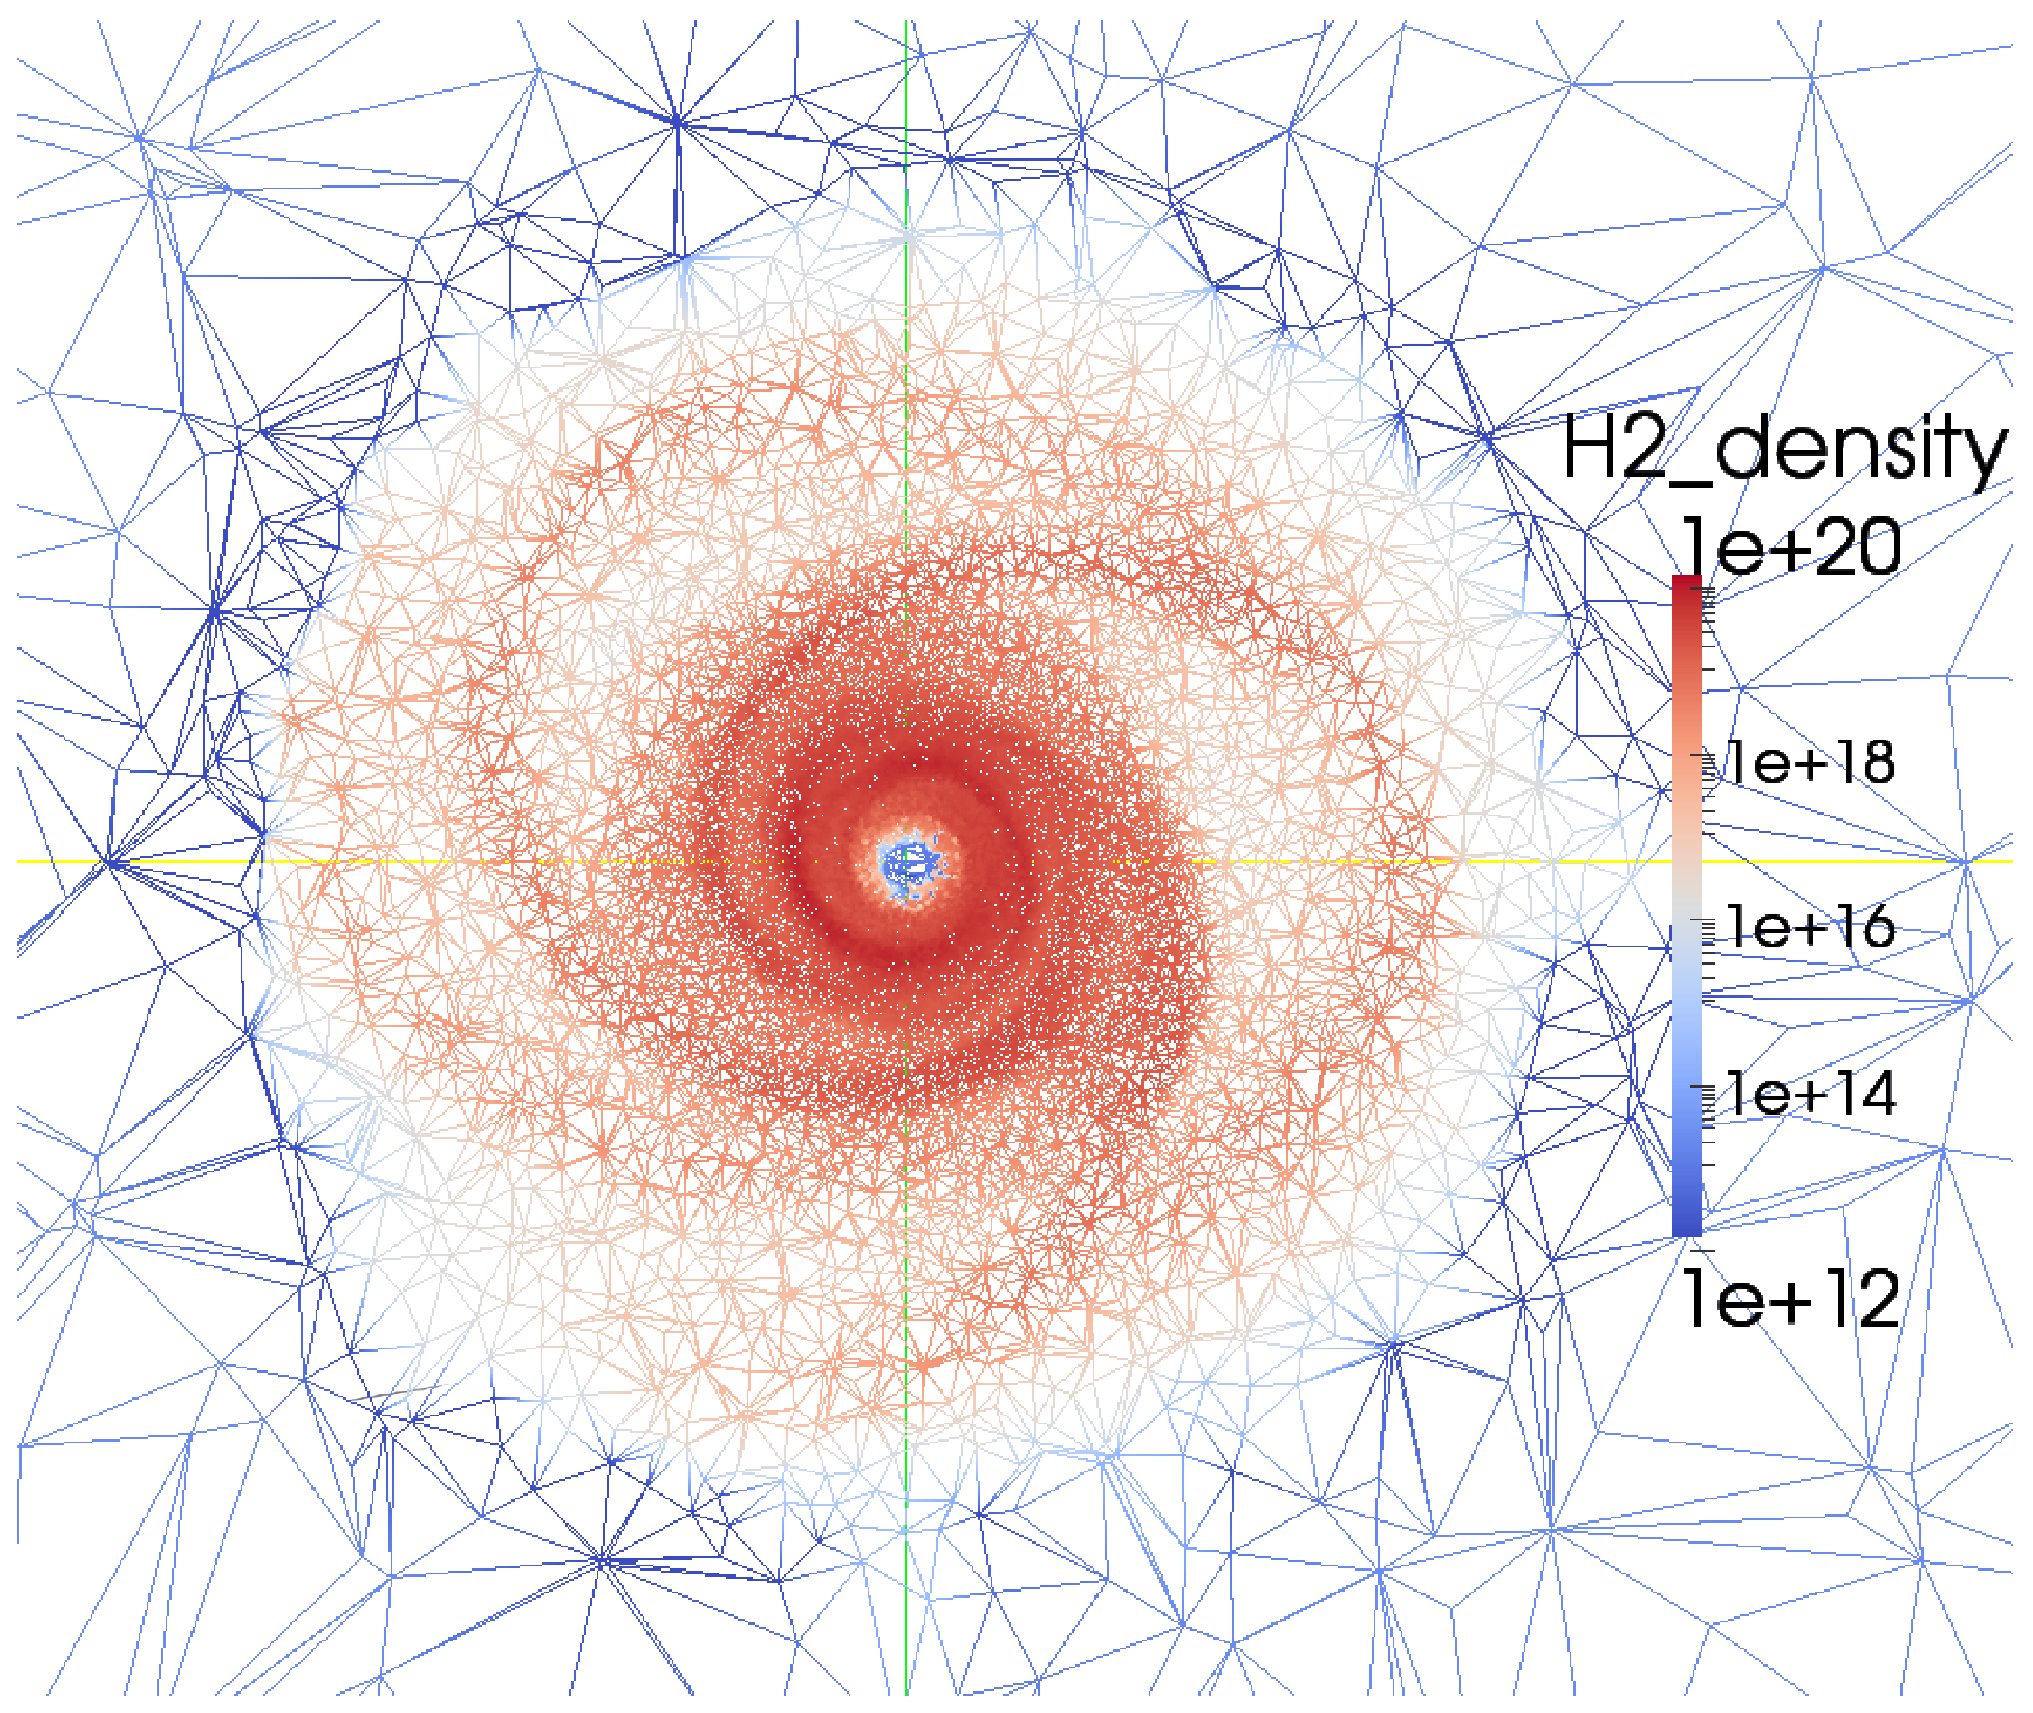
\includegraphics[width=84mm]{Figures/model/lime2.eps}%Lime_grid3.eps
 \caption{A plot of the points selected by the gridding process and the paths down which photons can propagate for points in the central r,$\theta$ plane. The points are colour coded by the density distribution (in m$^{-3}$, as used in LIME) and are more concentrated at small radii and in the most dense regions. The circular high density region in the centre is the disc model and is 128$\,$au in diameter.}
 \label{grid}
\end{figure}

\subsection{Grid construction} \label{subsec:gridding}
In order to construct the grid, candidate points are randomly selected from the volume to be simulated. These candidates then have their density and molecular density compared against a reference point in order to decide if the point is to be used in the grid or not. Candidate grid points are selected at random in cylindrical coordinates, linearly spaced in z and $\phi$ and logarithmically spaced in r. For each point to be selected, a random number $\alpha$ is drawn from the semi-open set [0,$\,$1) as a threshold. After selection of random coordinates, the hydrogen density and molecular density at the candidate point (n and m, respectively) are compared against the densities of a reference point on the inner edge of the disc (n$_0$ and m$_0$). If $\alpha<\left( \frac{n}{n_0} \right)^{0.3}$ or $\alpha< \left( \frac{m}{m_0} \right)^{0.3}$ then the point is selected for use, otherwise another r, $\phi$, z co-ordinate is selected and this becomes the candidate point. The function comparing the candidate point to the reference point and the candidate point distribution were selected empirically to sample all the scales while ensuring that the majority of points are located in the inner disc where the density is higher. 20\% of these points are forced to be at radii greater than $\sqrt{R_{min}R_{max}}$ (where $R_{min}$ and $R_{max}$ are the inner and outer radius of the model) in order to stop too many of the selected points clustering in the high density disc and leaving the envelope under sampled. In addition to this method of selection, 5\% of the points are linearly distributed in x, y and z with no bias with regards to density or abundance. This provides a minimum level of sampling for the large low density regions in the outer parts of the simulated volume. See figure \ref{points} for an example of the points distribution in r, z. \smallskip

\begin{figure}
 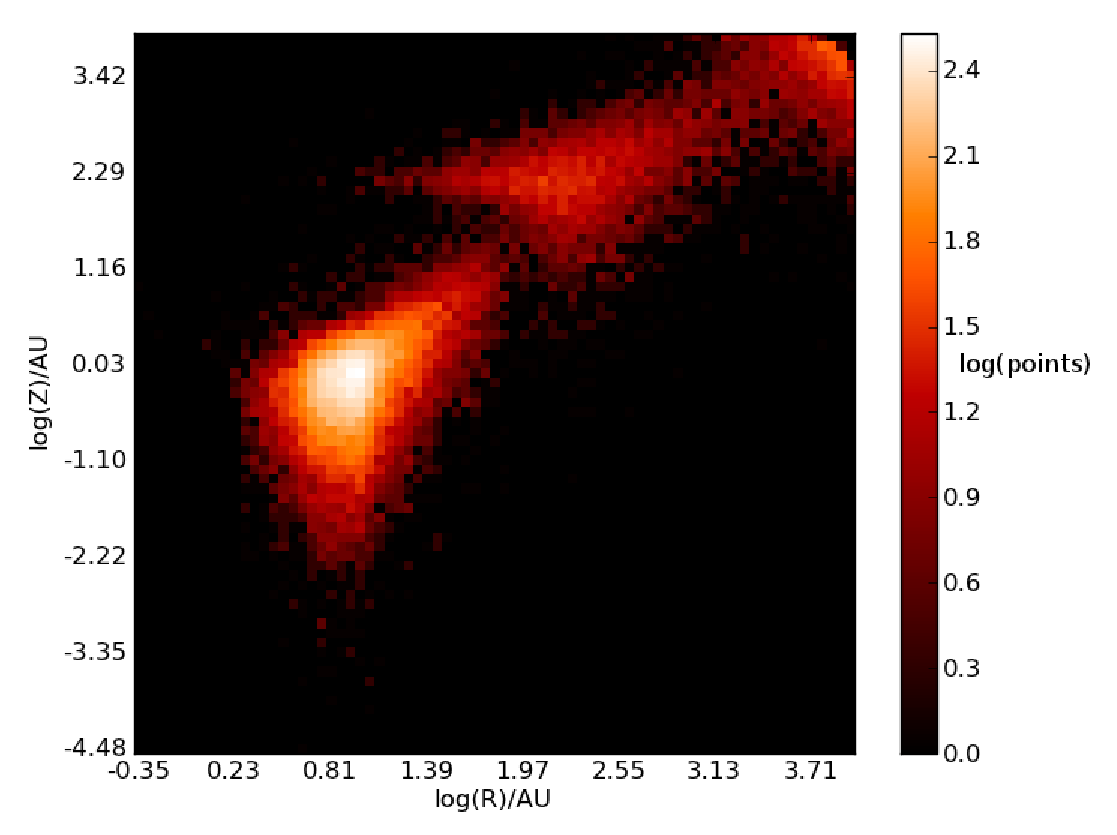
\includegraphics[width=84mm]{Figures/model/lime_points_rz_histo2.eps}
 \caption{A 2D histogram of the point distribution throughout the model. The disc and envelope can be seen as two separate entities which have to be sampled using different point distributions.}
 \label{points}
\end{figure}


\section{Model Results} \label{sec:model_results}

Simulations are limited to molecules for which we have abundances in both the disc and envelope, and also have calculated Einstein and collisional coefficients. In the envelope, the HCO$^+$ abundance profile follows the H$_2$O profile of L1544 \citep{Caselli2012}, scaled so the maximum is 1$\times$10$^{-8}$ (assuming, for simplicity, that photodissociation and freeze-out affect these two species in a similar way).For H$_2$CO, a step profile was considered, with a fractional abundance of 1.5$\times$10$^{-8}$ at radii greater than 0.04$\,$pc and 1.5$\times$10$^{-9}$ inside it \citep{Young2004}. For OCS we adopted a constant abundance of 1.9$\times$10$^{-9}$ \citep{Ren2011}. The C$^{17}$O abundance profile in the envelope follows the CO profile calculated for L1544 by KC2010, scaled by the 17O/16O elemental abundance. These estimates for the abundances in the envelope are simplistic, however, as seen in section \ref{alma_predictions}, the envelope contribution to the line is very narrow, and can be spectrally disentangled from the disc contribution.\smallskip

We focus on the frequency range available with ALMA, with particular attention to band 7, which offers the best trade off between resolution and sensitivity. Thus, we consider C$^{17}$O(3$\rightarrow$2), HCO$^+$(3$\rightarrow$2), OCS (26$\rightarrow$25) and H$_2$CO(4$_{04}\rightarrow$3$_{03}$).  The frequencies and upper level energies of these transitions are in table \ref{sigmas}. The results presented in this section are limited to those lines which show detectable emission/absorption which can be used to trace either spiral structure or rotation.\smallskip

%We considered C$^{17}$O 3$\rightarrow$2 at 337.1$\,$GHz with an upper energy level of $E_u$=32.3K, HCO$^+$ 3$\rightarrow$2 at 267$\,$GHz and $E_u$=25.7K, OCS 26$\rightarrow$25 at 316$\,$GHz and $E_u$=205K and H$_2$CO 4$_{04}\rightarrow$3$_{03}$ at 290$\,$GHz and $E_u$=34.9K.\smallskip

To simulate observations, the model was placed at roughly the distance of nearby low-mass star forming regions (100$\,$pc). The inlination angle was varied from 15$^\circ$ to 75$^\circ$ to edge on, we will consider the 30$^\circ$ case as a 'typical' inclination with the 15$^\circ$ inclination discussed in section \ref{alma_predictions}, the other inclinations simulated are shown in appendix \ref{other_inc}. From these simulated observations, integrated intensity maps, intensity weighted velocity maps and position velocity diagrams were created. The integrated intensity and intensity weighted velocity maps (figures \ref{sim_all} and \ref{mom0_maps}) were created by integrating between -12.5 to -0.5$\,$km$\,$s$^{-1}$ and +0.5 to +12.5$\,$km$\,$s$^{-1}$ to avoid being dominated by the contribution from the envelope. This can be seen in some PV diagrams  (Figure \ref{pvs}) as the strong absorption feature at all positions around zero velocity. Moment 1 maps are shown with a cut-off of 3$\sigma$ as described in section \ref{sec:alma_predictions}.\smallskip

\begin{figure}
 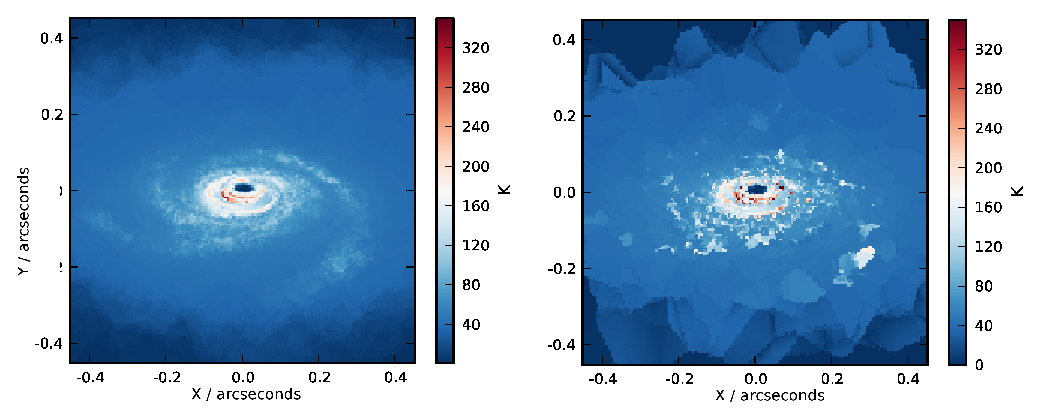
\includegraphics[width=84mm]{Figures/sim/continuum.eps}
 \caption{{\bf Left:}A 300$\,$GHz continuum image of the model, created from the average of ten LIME runs. {\bf Right:} the output of a single radiative transfer simulation, with artifacts due to finite gridding.}
 \label{averages}
\end{figure}

\begin{figure*}
 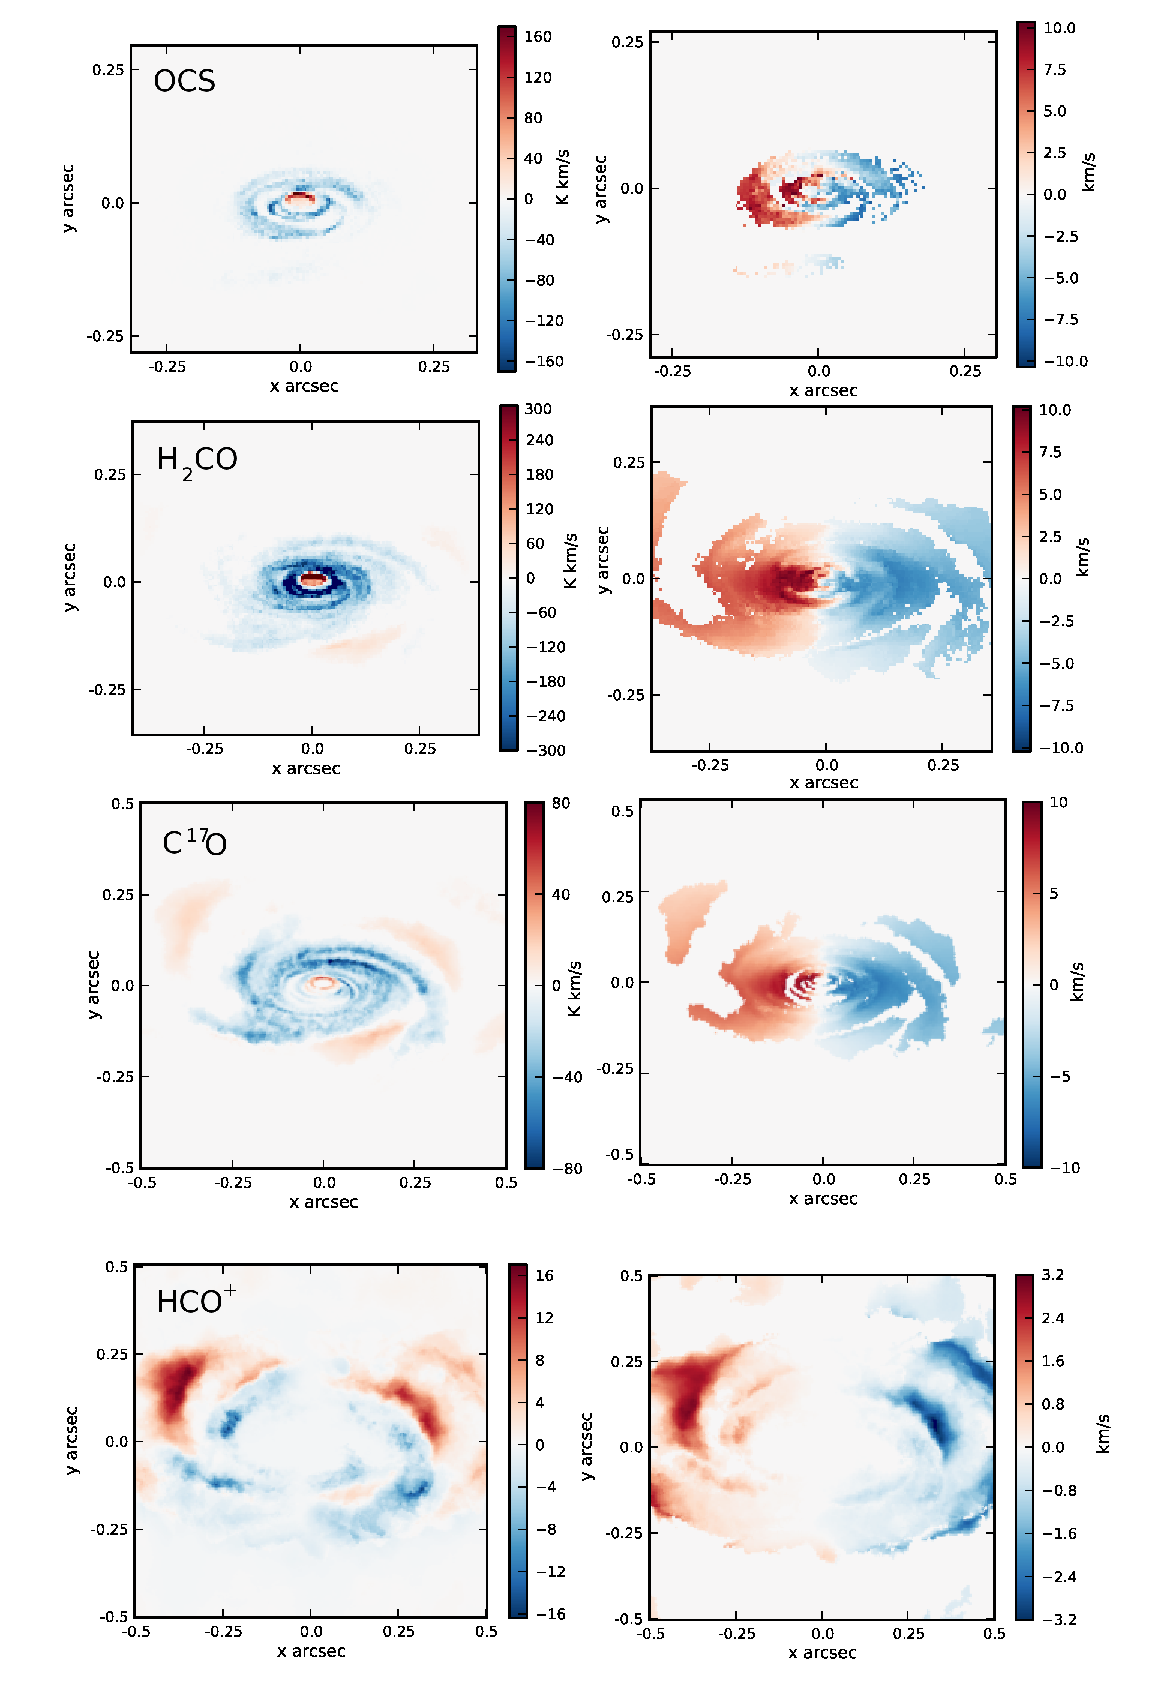
\includegraphics[width=150mm]{Figures/sim/imageALL_30deg_all.eps}
 \caption{{\bf Left:} Continuum subtracted integrated intensity maps. {\bf Right:} Intensity weighted velocity maps. The spiral structure in different regions of the disc is highlighted by looking at different molecular lines. From top to bottom the lines displayed are: OCS 26$\rightarrow$25, H$_2$CO 4$_{04}$$\rightarrow$3$_{03}$, C$^{17}$O 3$\rightarrow$2 and HCO$^+$ 3$\rightarrow$2. All maps are integrated over -12.5 to -0.5 and 0.5 to 12.5 km$\,$s$^{-1}$ in order to avoid the envelope contribution.}
 \label{sim_all}
\end{figure*}


OCS 26$\rightarrow$25 traces only the innermost 20$\,$au of the disc and can be used to examine the central regions (figure \ref{sim_all}). As OCS is not seen in outflows (e.g. \citealt{Stanke2007}, \citealt{VDTak2003}) it can be used to view rotation of the central part of the disc without risk of contamination from emission from shocked material along the outflow. The OCS line, which has the highest upper energy level among the selected transitions, traces the hottest and densest regions of the disc. As a result, the innermost spiral structure is best seen in OCS (26 - 25), as shown in figure \ref{sim_all}. The majority of the OCS line is visible in absorption against the bright continuum emission from the disc mid-plane. The exception to this is towards the centre of the disc where the hole in the hot, dense mid-plane means that there is little continuum to be absorbed. However, because of the presence of the protostar and other hot material within 2$\,$au of the protostar, not considered in our simple model, we expect absorption to also be observed toward the central region of the disc.\smallskip

The abundance of the H$_2$CO molecule traces the spiral structure of the inner $\sim$40$\,$au of the disc, which can be seen in the integrated intensity map and its rotation is detected out to larger radii than is possible with the OCS line (figure \ref{sim_all}). As with the OCS line, the majority of the H$_2$CO 4$_{04}\rightarrow$3$_{03}$, is seen in absorption against the disc mid-plane continuum, with the central region seen in emission. Unlike the OCS however, the H$_2$CO extends out to large enough radii to be present in the voids between the outer parts spiral arms. In these regions, the H$_2$CO line can be seen in emission.\smallskip

The fractional abundance of C$^{17}$O is constant at 2$\times$10$^{-8}$ across the disc, so that the selected C$^{17}$O line is the most accurate in reproducing the physical structure of the disc. Like H$_2$CO, C$^{17}$O shows emission in voids between spiral arms. The C$^{17}$O line is visible from the inner edge of the disc to its outer edge. Like OCS, C$^{17}$O is not seen in outflows \citep{Yildiz2012}, so we do not expect contamination.\smallskip

HCO$^+$ in unique in the molecules simulated in I2011 in that it traces only the outer regions of the disc, and so can be used to look at the extended velocity and physical structure. In figure \ref{sim_all} we can see that the HCO$^+$ line shows the outer edges of the spiral arms in absorption, but it also shows emission from the diffuse gas further out in the disc. This allows the velocity structure of the disc to be measured out to larger radii. This allows constraints to be placed on the rotation of the disc out to larger radii than with other molecules. 


\section{Predictions for ALMA} \label{sec:alma_predictions}

In order to make predictions on the observability of the synthetic brightness maps, the Common Astronomy Software Applications package (CASA) was used to simulate their observation with the completed ALMA in the 26th most extended configuration (out of a total of 28), with the longest baseline of 14.4km and giving beam sizes between 0.02 and 0.03 arcseconds at the selected frequencies, giving a beam size close to the size of the spiral structure in the disc. As the weakest lines studied in the model are of the order of 0.1-0.2$\,$mJy$\,$beam$^{-1}$ at this resolution, sensitivities of the order of 0.02$\,$mJy$\,$beam$^{-1}$ are required. This implies around 6 hours of integration time. The exact sensitivities are given in Table \ref{sigmas}.
\begin{table*}
  \centering
  \begin{minipage}{80mm}
    \caption{Line sensitivities obtained with ALMA after 6 hours integration time with velocity resolution of $\sim$400$\,$ms$^{-1}$. As calculated by the ALMA on-line sensitivity calculator.}
    \label{sigmas}
    \begin{tabular}{c||c|c|c|c}
      \hline
      Species & Transition & Frequency & Upper energy level & Sensitivity\\
      \hline
      C$^{17}$O & 3$\rightarrow$2 & 337.06GHz & 32.3$\,$K & 0.0270$\,$mJy$\,$beam$^{-1}$ \\
      OCS & 26$\rightarrow$25 & 316.15GHz & 25.7$\,$K & 0.0275$\,$mJy$\,$beam$^{-1}$ \\
      HCO$^+$ & 3$\rightarrow$2 & 267.56GHz & 205$\,$K & 0.0176$\,$mJy$\,$beam$^{-1}$ \\
      H$_2$CO & 4$_{04}\rightarrow$3$_{03}$ &  290.62GHz & 34.9$\,$K & 0.0228$\,$mJy$\,$beam$^{-1}$ \\
      \hline
    \end{tabular}
  \end{minipage}
\end{table*}
In order to clean the images, which featured mainly absorption, the sky model used was the output of the LIME simulations with the continuum subtracted and then the spectrum inverted. The simulated images were cleaned down to a 3$\sigma$ level with $\sigma$ (the sensitivity) given in table \ref{sigmas}.\smallskip

\begin{figure}
 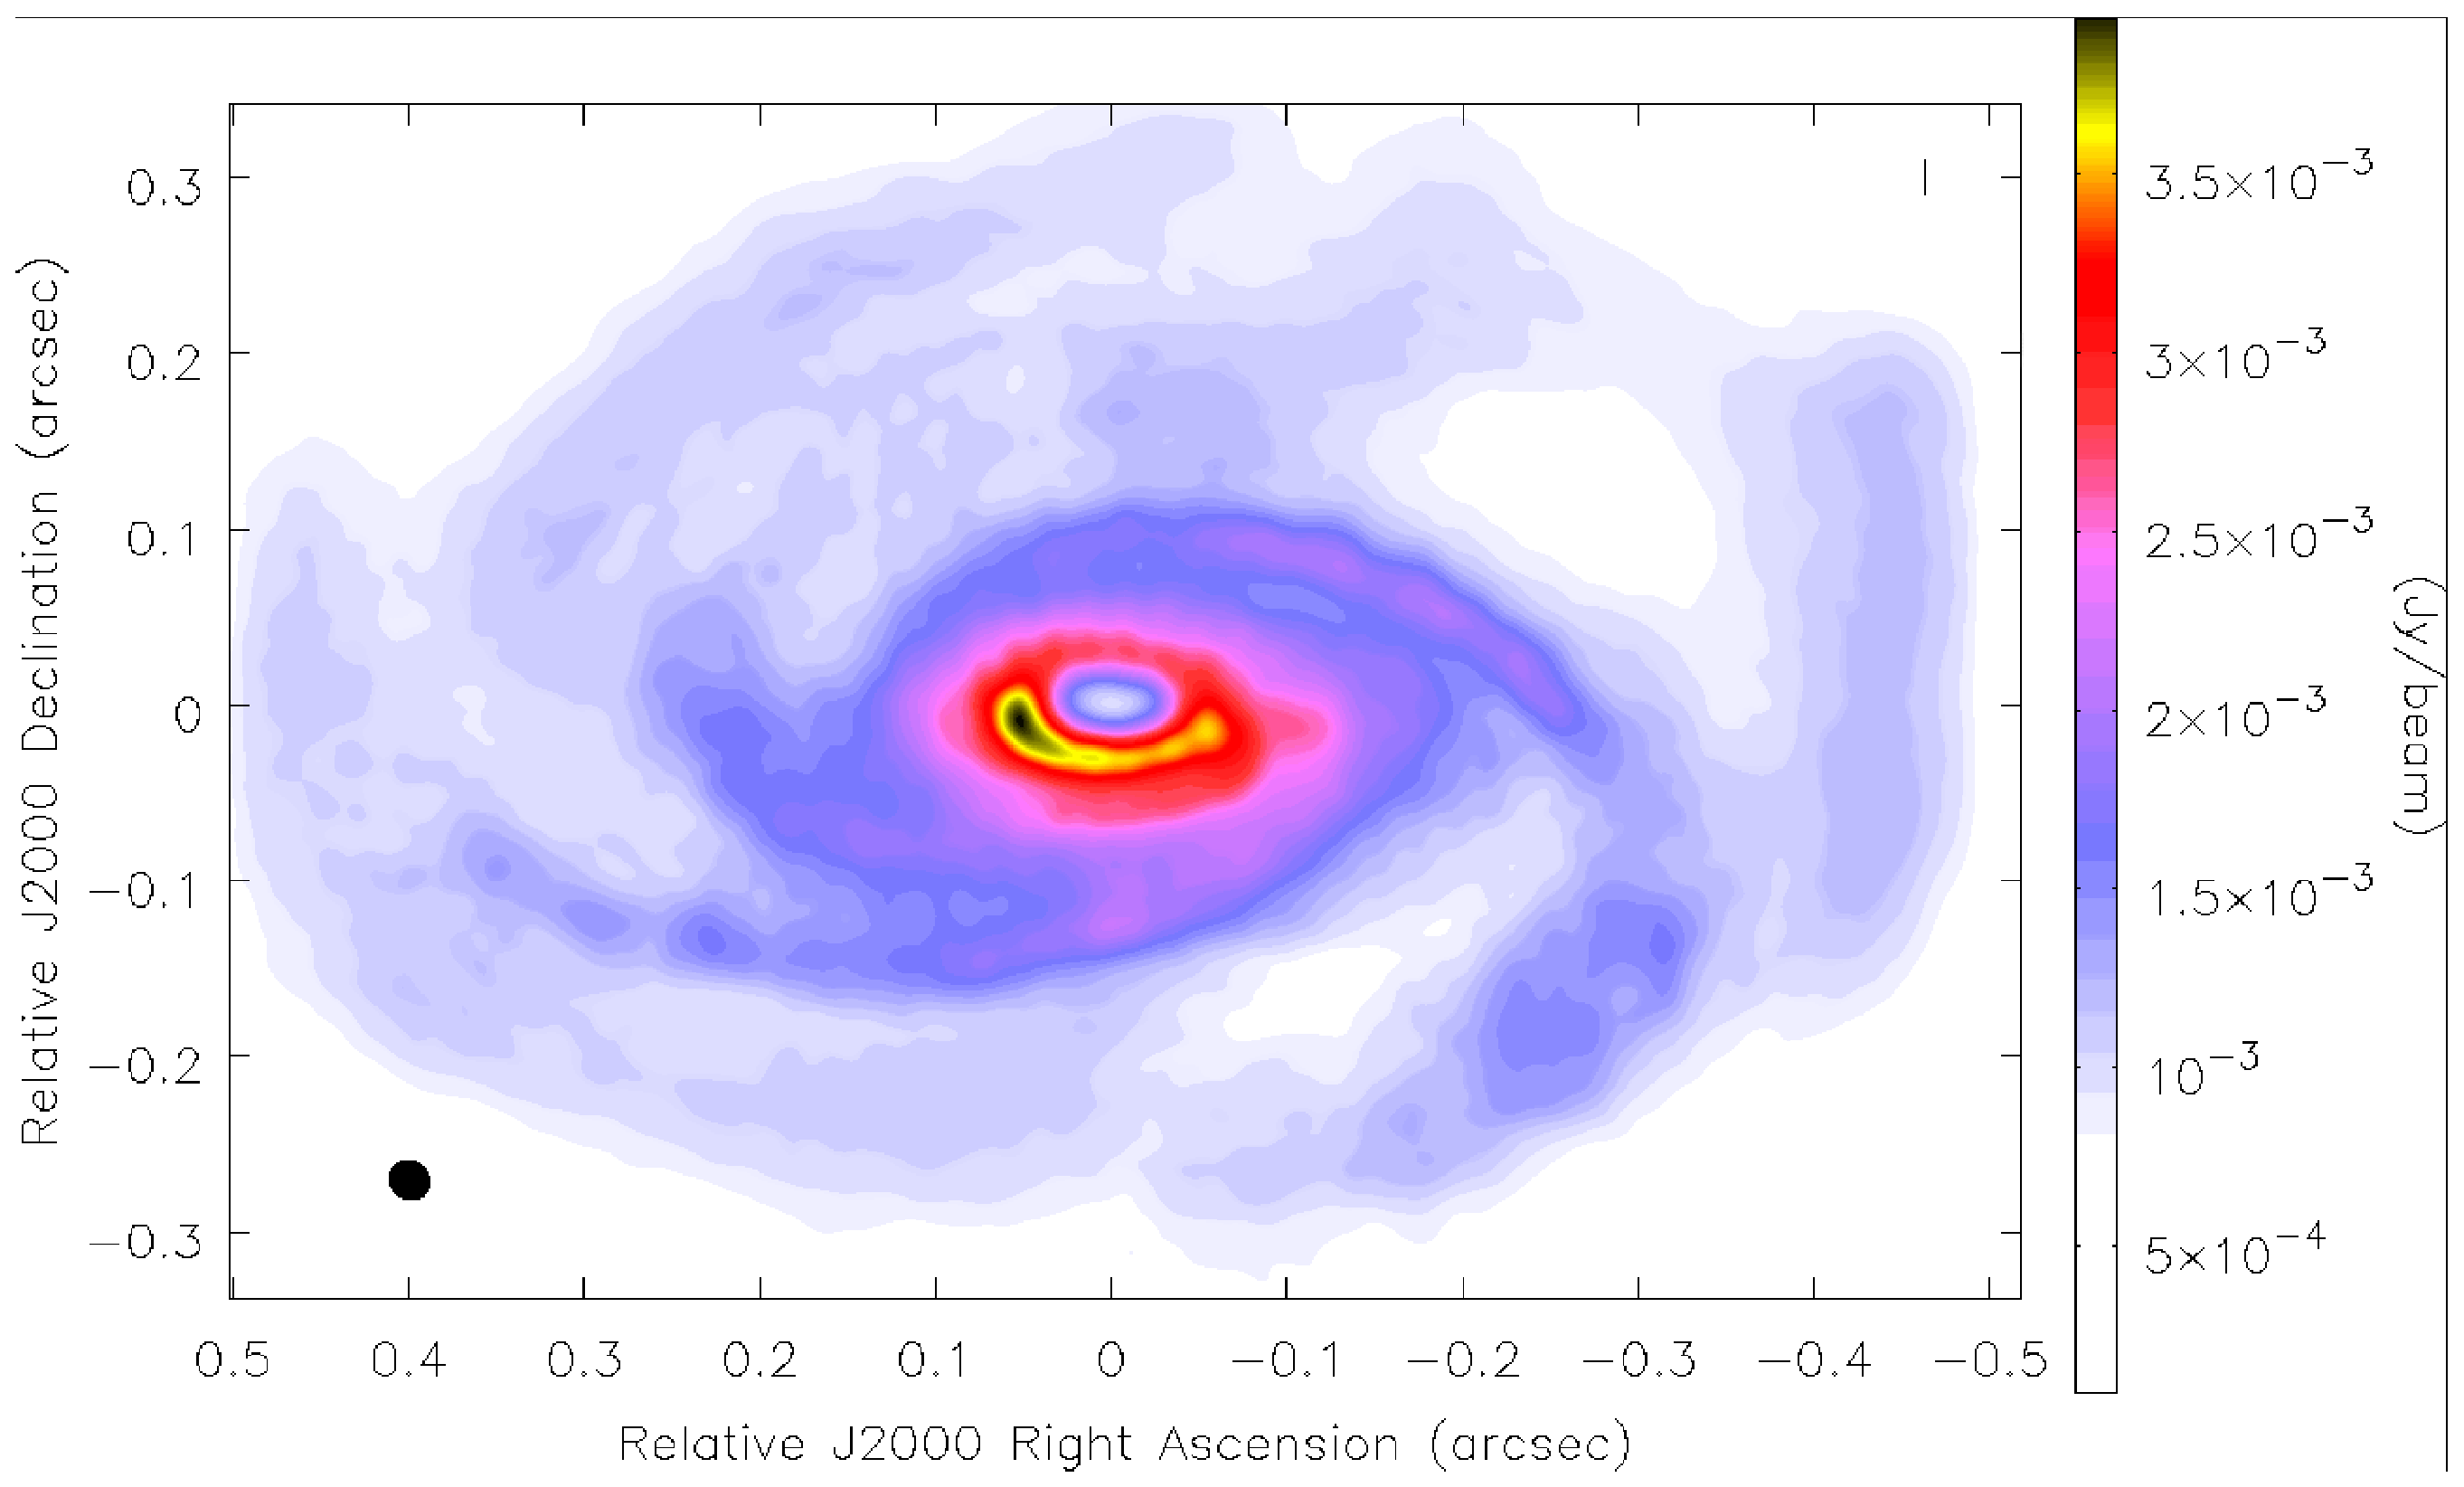
\includegraphics[width=84mm]{Figures/sim/casa_cont_300GHz_invert.eps}

 \caption{CASA simulation of the continuum emission of the model at 300GHz, using the same ALMA configuration as used for the molecular lines. The size of the beam at 300GHz is shown in the lower left corner.}
 \label{continuum}
\end{figure}

\begin{figure*}
 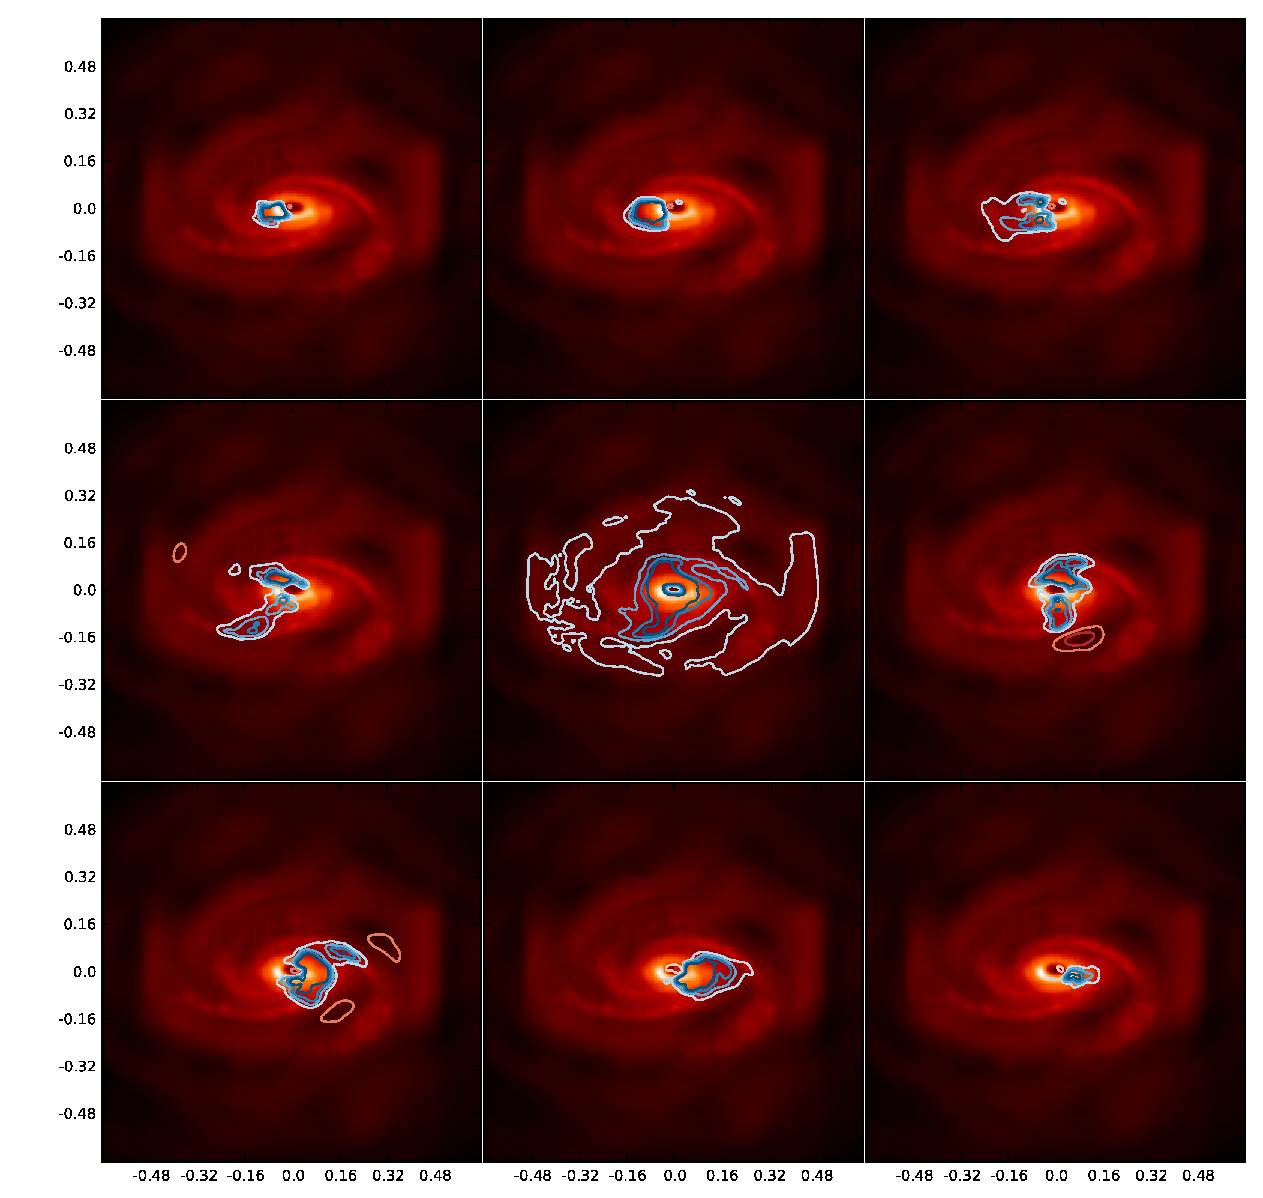
\includegraphics[width=168mm]{Figures/sim/channel_map-1.eps} 
 \caption{H$_2$CO 4$_{04}\rightarrow$3$_{03}$ channel maps as simulated by CASA. The contours start at 0.35 mJy$\,$beam$^{-1}\,$km$\,$s$^{-1}$  and are in steps of 0.35 mJy$\,$beam$^{-1}\,$km$\,$s$^{-1}$ (absorption in blue, emission in red). Overlaid on the 1mm continuum emission. Each map integrates over 2.4 km$\,$s$^{-1}$ with the top left from -10.8 to -8.4 km$\,$s$^{-1}$ to the bottom left ranging from 8.4 to 10.8 km$\,$s$^{-1}$}
 \label{h2co_chanmap}
\end{figure*}

Figure \ref{continuum} Shows the 1mm continuum emission and beam size in this configuration of ALMA. The spiral structure of the disc is clearly visible at this inclination and will be clearer the closer the disc is to being face on. \smallskip 

Figure \ref{h2co_chanmap} shows a channel map of the H$_2$CO 4$_{04}\rightarrow$3$_{03}$ line overlaid on the 1$\,$mm continuum emission. From this it can be seen that the absorption features trace the disc spiral structure whilst the line emission emanates from gaps in the outer disc, where there is less continuum to be absorbed. The central pannel is domminated by the envelope contribution, causing stron absorption through out the disc. The other pannels show the line following a rotation profile distorted by the presence of the spiral arms. \smallskip


\begin{figure*}
 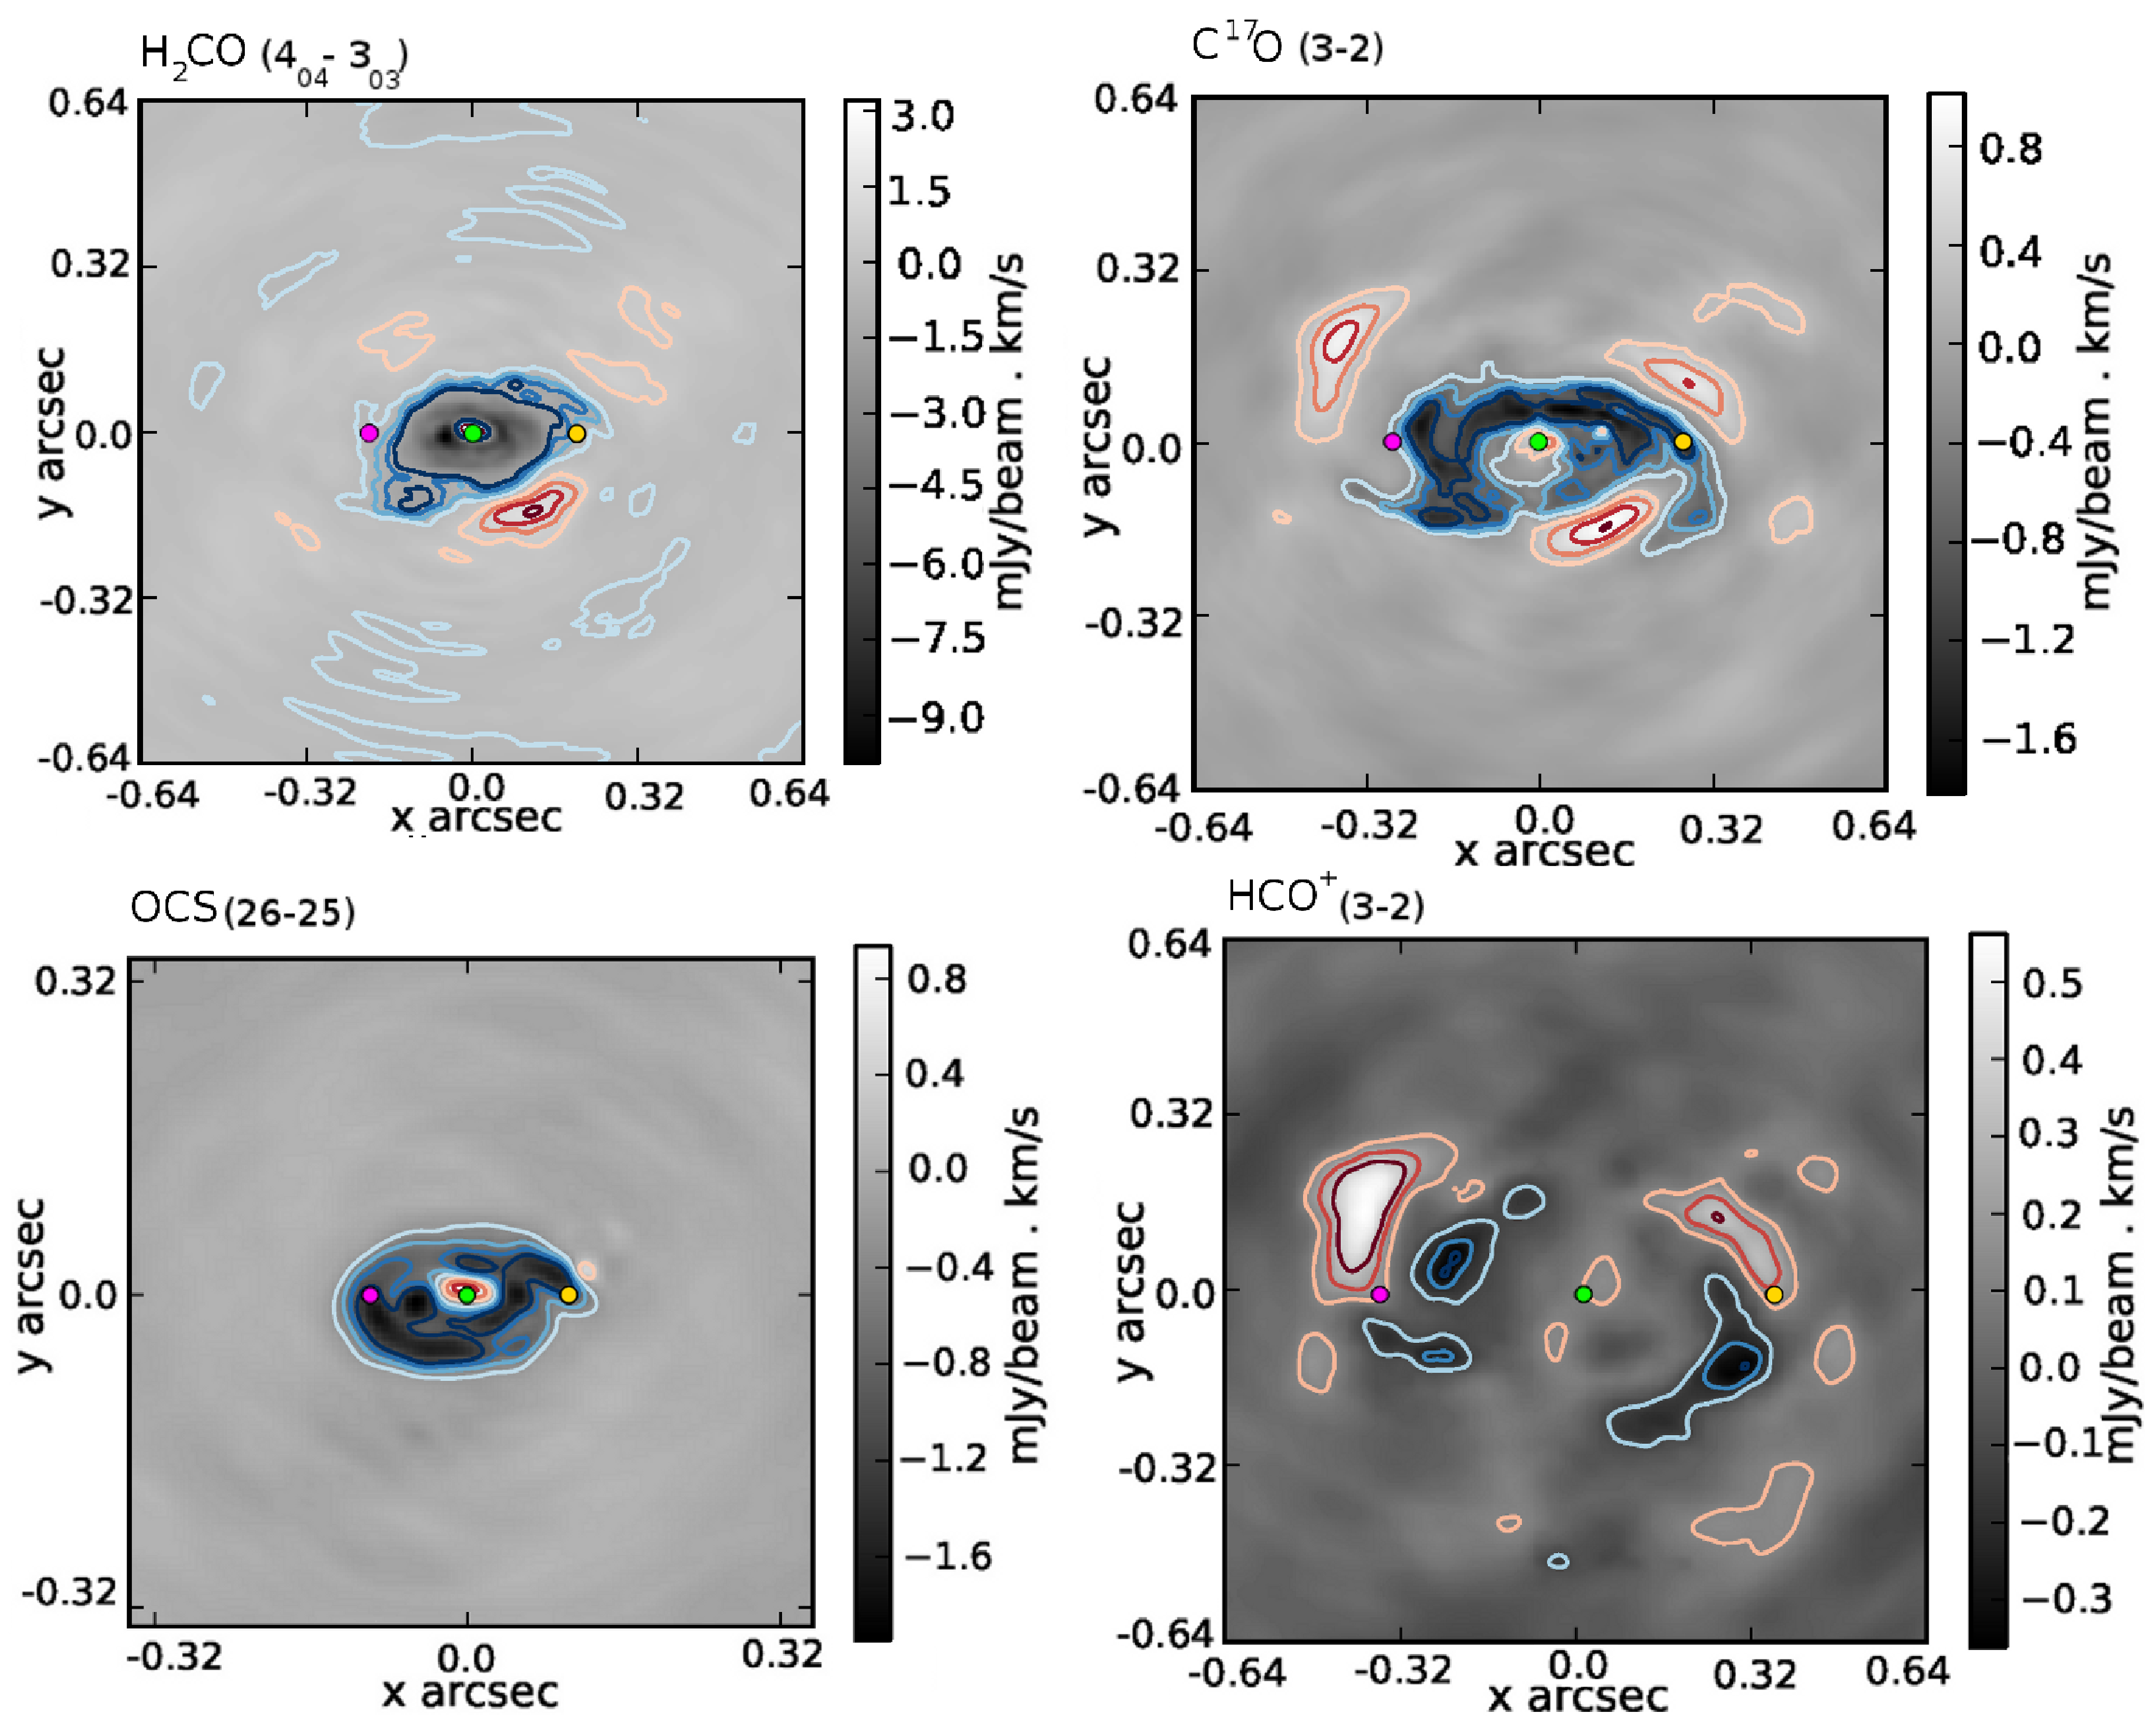
\includegraphics[width=168mm]{Figures/sim/casa_all_30deg_contSub_dots.eps}
 \caption{Integrated intensity maps for the simulated observations of: {\bf Top Left:} H$_2$CO 4$_{04}\rightarrow$3$_{03}$, {\bf Top Right:} C$^{17}$O 3$\rightarrow$2, {\bf Bottom Left:} OCS 26$\rightarrow$25 and {\bf Bottom Right:} HCO$^+$ 3$\rightarrow$2. Contours start at 3$\sigma$ and increasing in intervals of 3$\sigma$ for each of the maps except the H$_2$CO which starts at 5$\sigma$ and increases in intervals of 5$\sigma$. Emission is in red contours, absorption in blue. The dots refer to the spectra shown in figure \ref{spectra}.}
\label{mom0_maps}
\end{figure*}

Figure \ref{mom0_maps} shows the simulated integrated intensity maps, which demonstrates how lines from different species allow observations to trace different regions of the disc, from the OCS line tracing the innermost regions, to the HCO$^+$ line showing the outer regions which are less bright in the continuum. ALMA has enough resolution and sensitivity to see spiral structure clearly in continuum emission but also in CO isotopologues and marginally in H$_2$CO. The different molecules can be seen to be tracing different regions of the disc\smallskip

\begin{figure}
 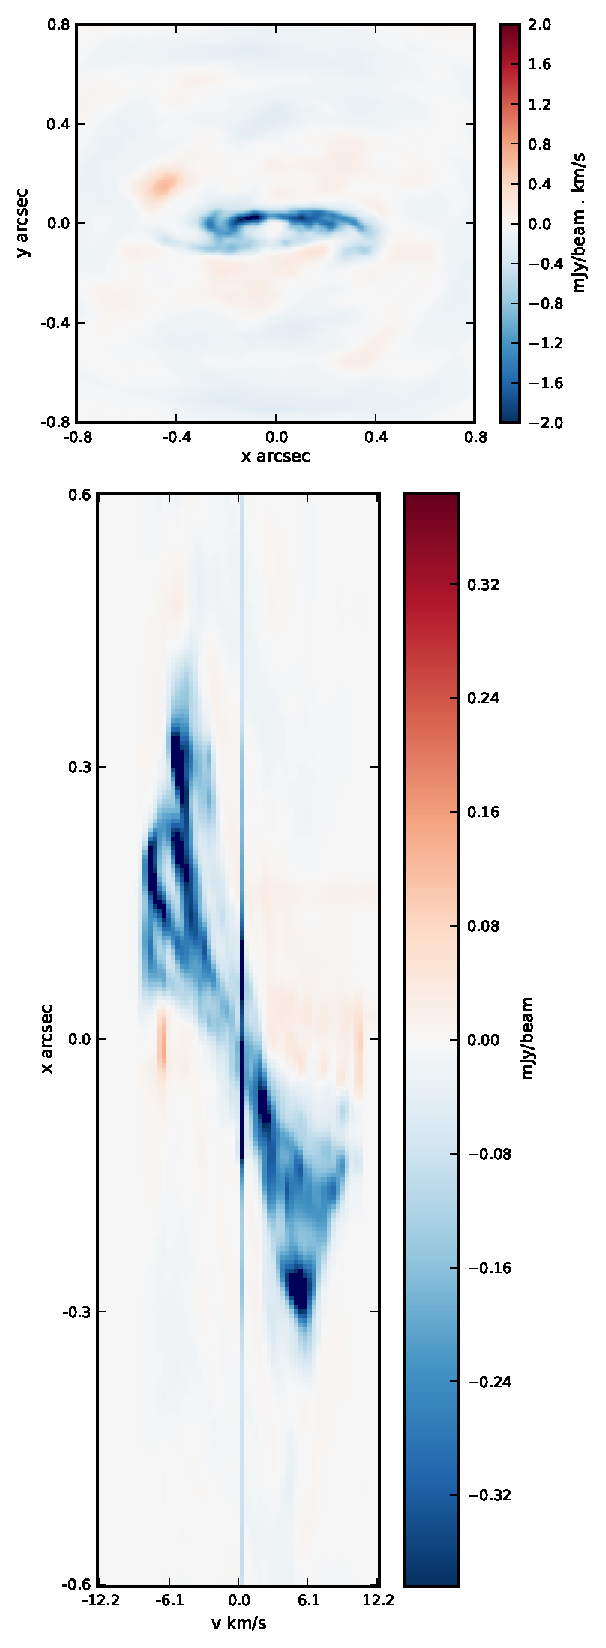
\includegraphics[width=63mm]{Figures/sim/casa_C17O_15deg_all.eps}

 \caption{CASA simulation of the C17O 3$\rightarrow$2 line inclided at 15$^\circ$ to edge on {\bf Top:} integrated intensity map. {\bf bottom:} position velocity diagram. In the position velocity diagram the spiral structures can be seen as narrow finger-like structures extending from the origin.}
 \label{15deg}
\end{figure}

%\begin{figure}
%  \centering
%  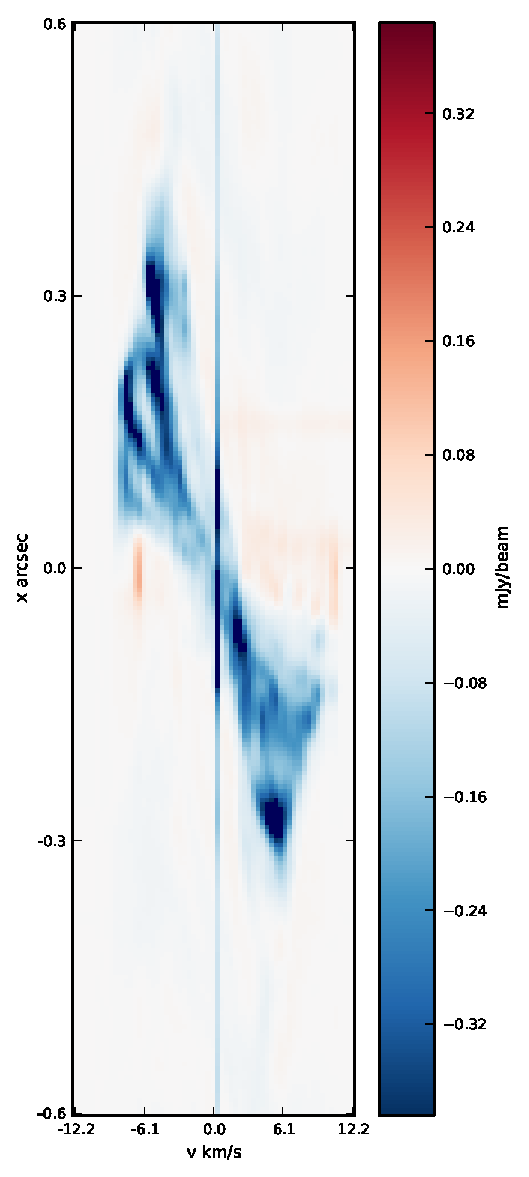
\includegraphics[width=42mm]{Figures/sim/casa_C17O_15deg_PV.eps}
  
%  \caption{CASA simulation of the position velocity diagram of the C17O 3$\rightarrow$2 line inclided at 15$^\circ$ to edge on.}
%  \label{15deg_pv}
%\end{figure}


\begin{figure*}
 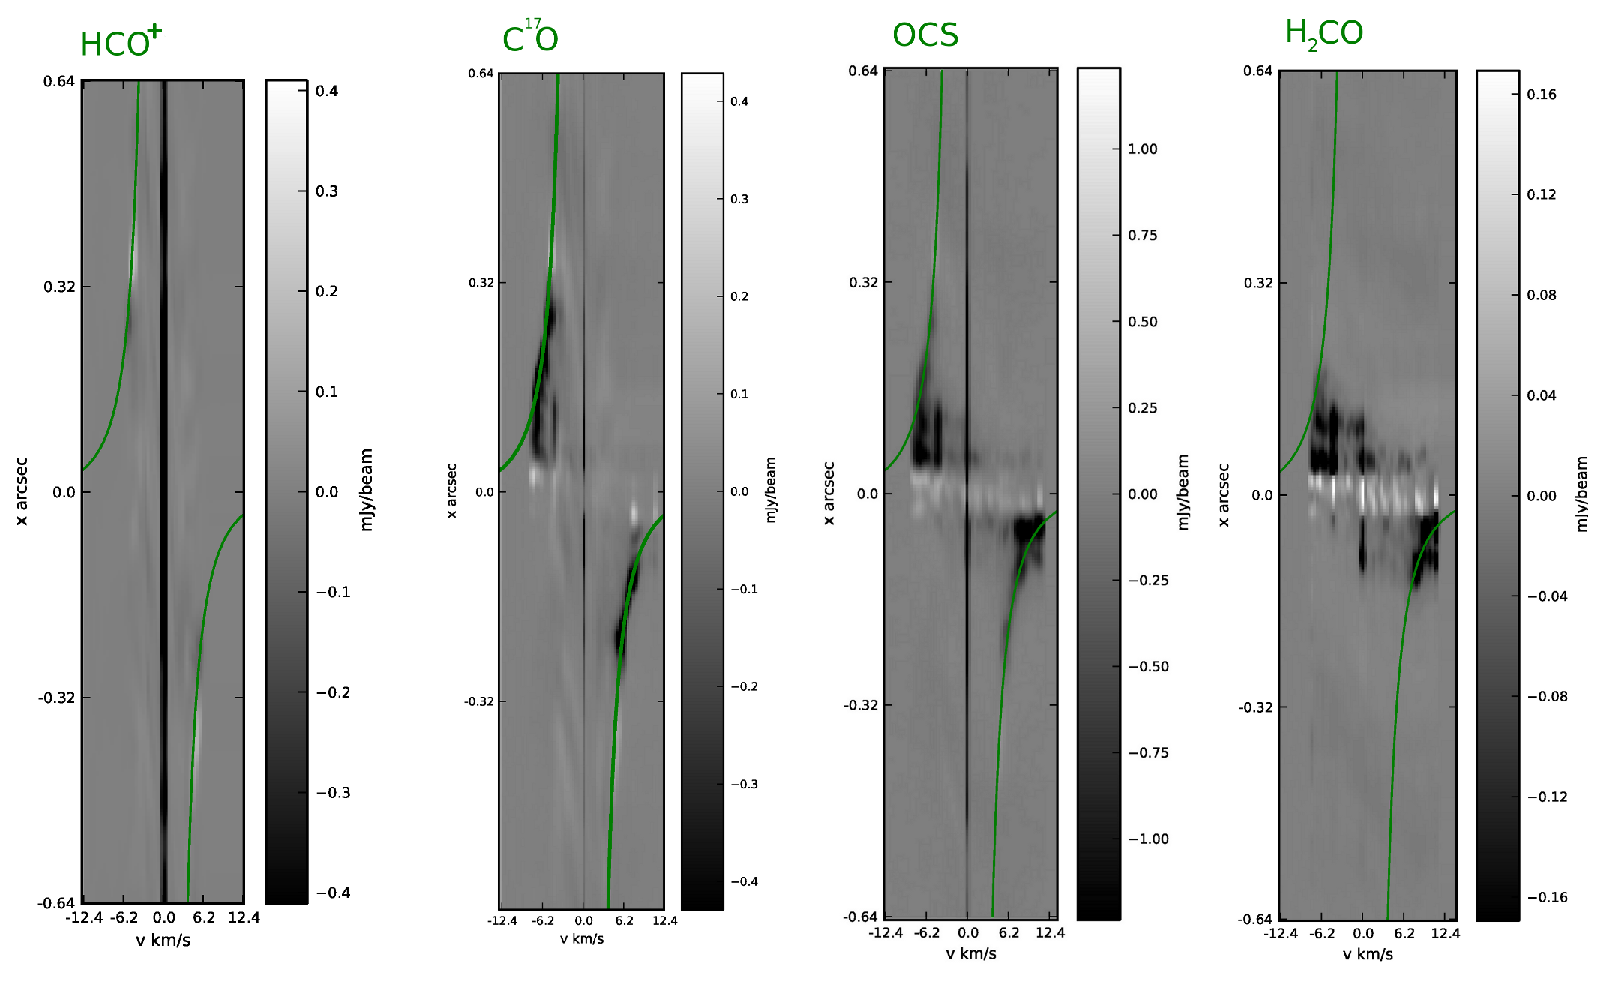
\includegraphics[width=180mm]{Figures/sim/casa_all_30deg_PV_rotCurve_small.eps}
 \caption{Position velocity diagrams for each of the lines simulated with CASA. The green curve on each diagram is the best fit curve to the azimuthally averaged rotation profile from figure 4.}
 \label{pvs}
\end{figure*}

Figure \ref{pvs} shows position-velocity diagrams of the lines simulated, allowing us to reconstruct the rotation of the disc. The green curves in each panel of figure \ref{pvs} display the best fit rotation curve of the physical model (see figure \ref{velocity}), showing that the rotation profile of the disc can be well constrained using kinematic information gathered from species tracing different regions of the disc.\smallskip

\begin{figure*}
 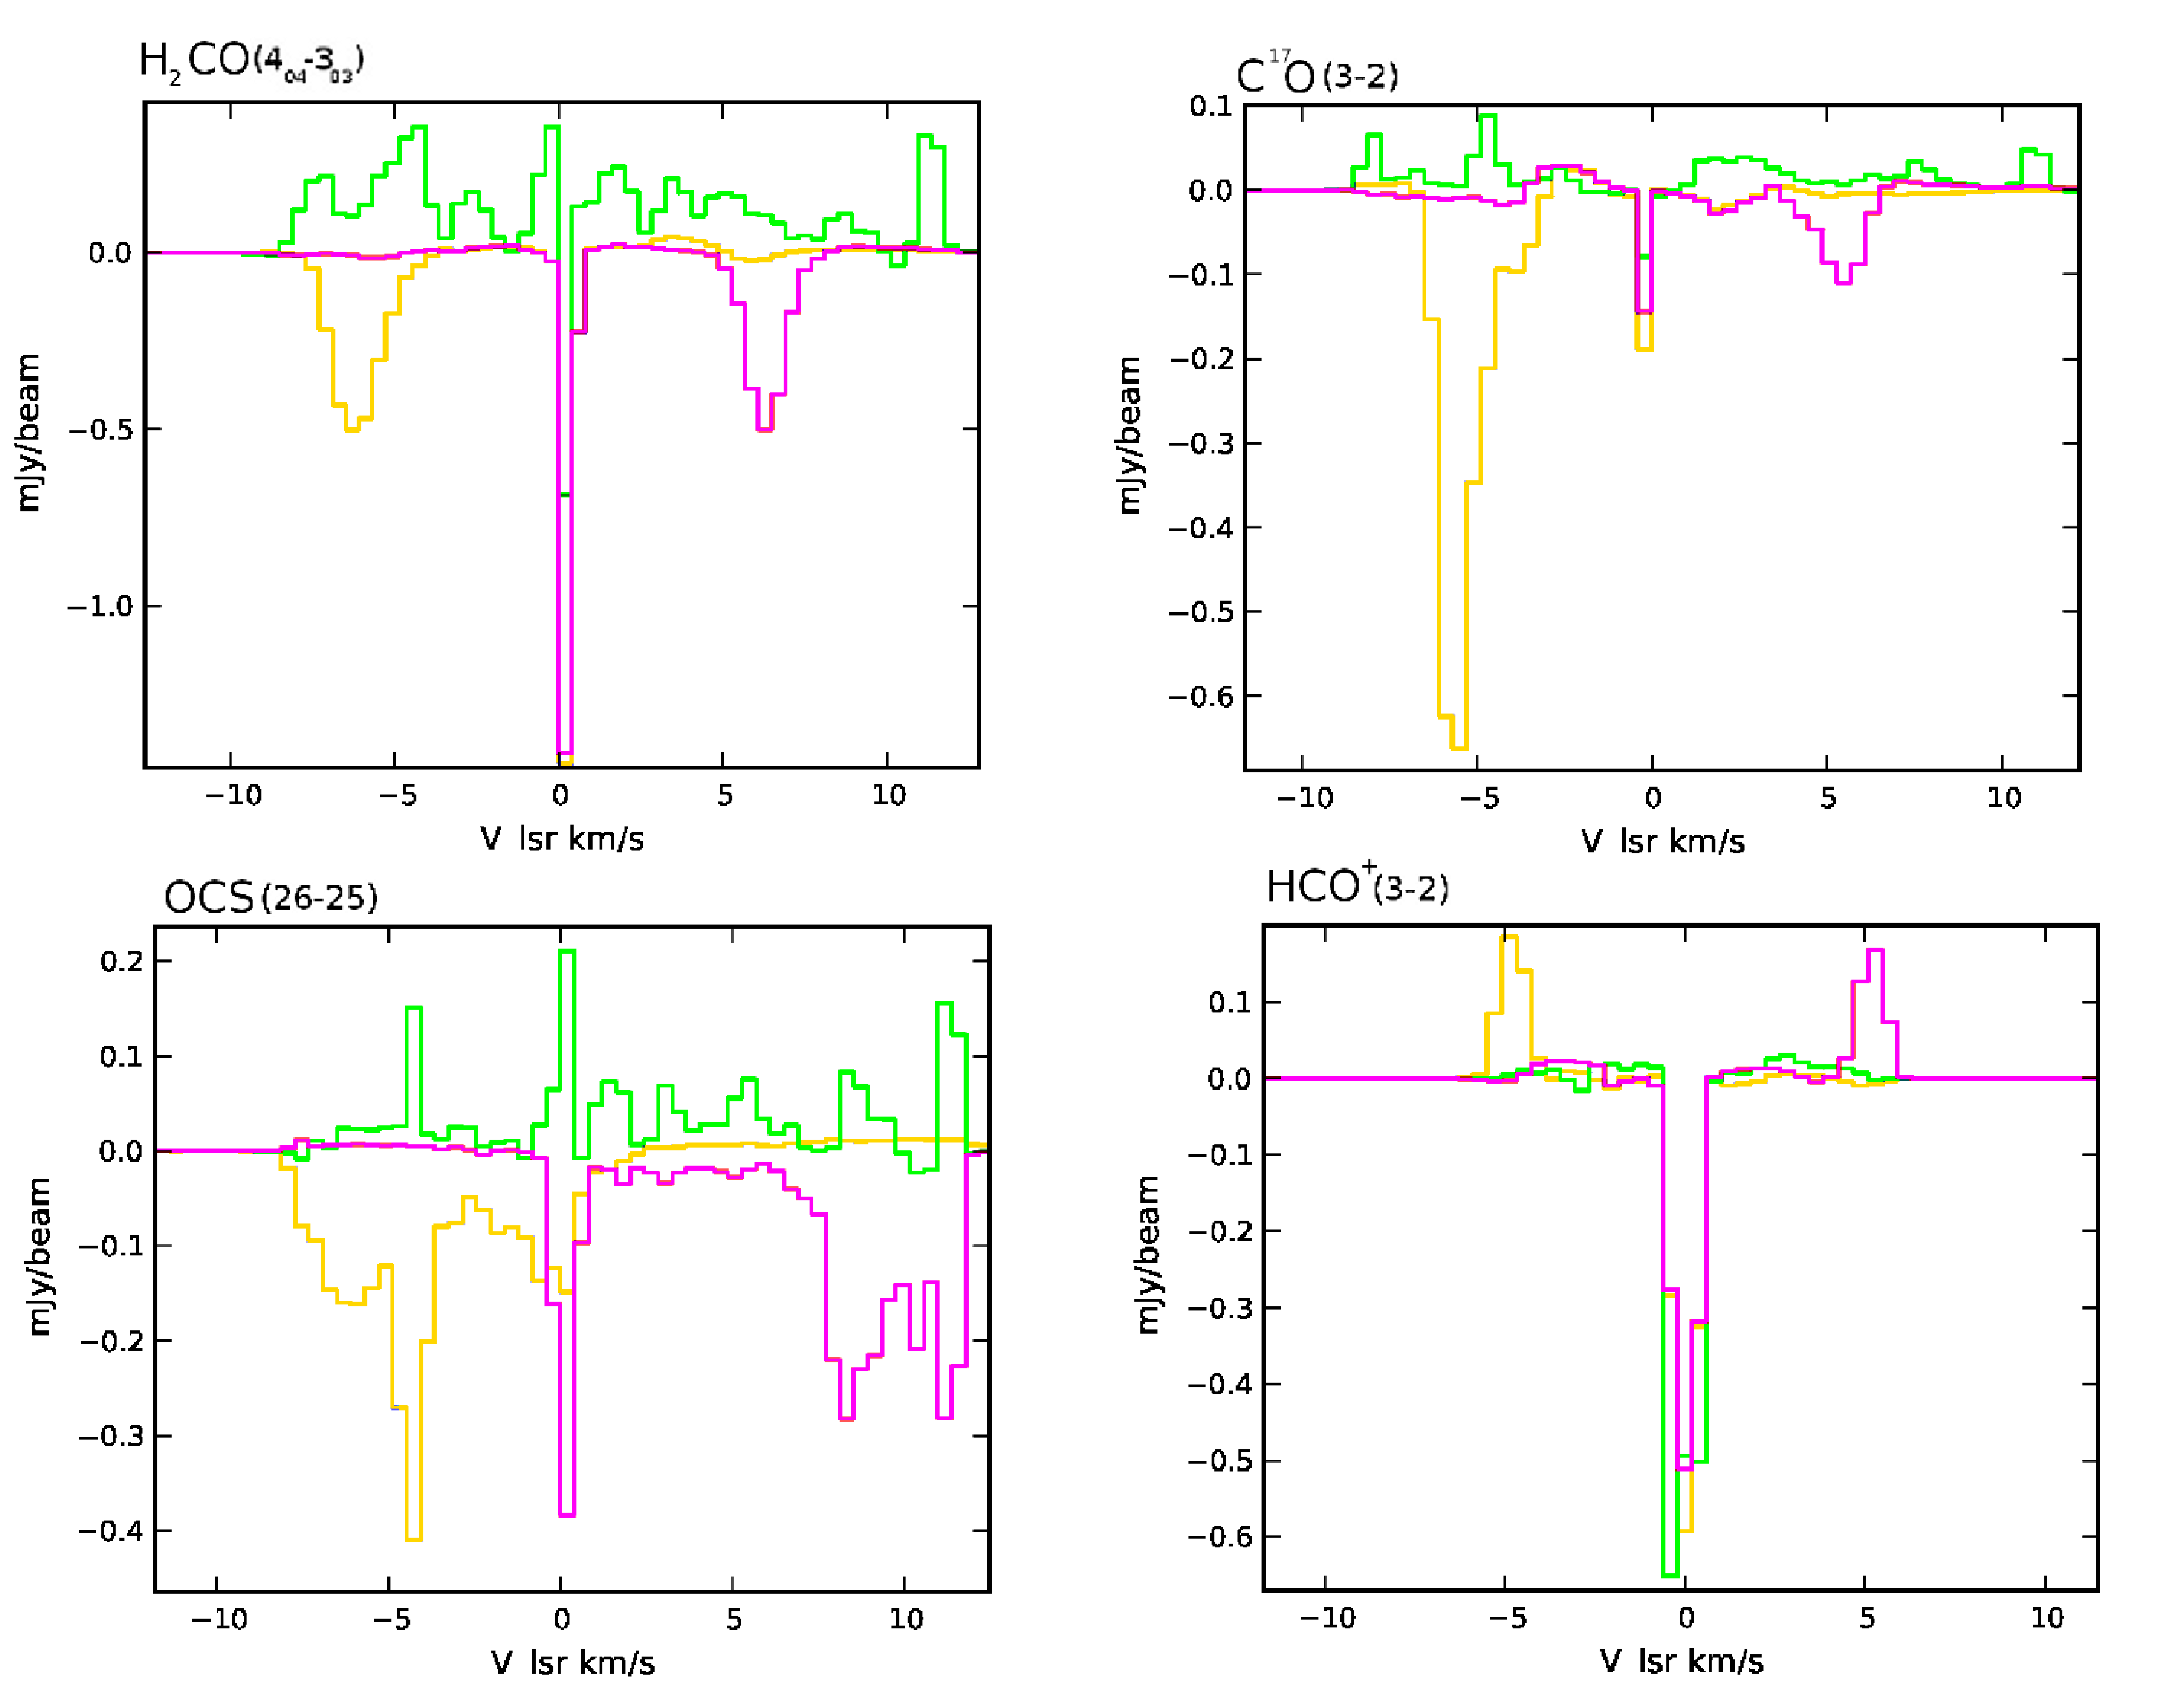
\includegraphics[width=168mm]{Figures/sim/casa_all_spectra2.eps}
 \caption{Simulated spectra for each of the selected transitions at the positions indicated by the coloured dots in figure \ref{mom0_maps}, the pink, green and cyan curves are taken from the locations marked by the dot of the same colour. In each diagram, the three spectra are taken from three positions on the Y=0 axis, one is at X=0 (green) and the other 2 are from x=$\pm$ N (plus blue, minus red) where N is the distance from the centre: 10 au for OCS, 20 au for H$_2$CO, 28 au for C$^{17}$O, 38 au for HCO$^+$.}
 \label{spectra}
\end{figure*}

Figure \ref{spectra} shows spectra from the lines simulated, one from the centre of the image and one on each side of the disc along the Y=0 axis. As with all the CASA simulated images, these spectra have a total bandwidth of 938$\,$MHz, giving velocity resolutions of between 418 and 527 ms$^{-1}$. The most notable thing about these spectral features is that they are not symmetric about the disc centre. For example, C$^{17}$O(3$\rightarrow$2) has a significantly stronger blueshifted absorption, due to the presence of a spiral arm along the same line of sight. In the OCS lines, the two sides are not moving with equal velocities and the line widths and shapes are markedly different. These can be attributed to the non-axisymmetric nature of the model.

\section{Conclusions} \label{sec:discussion}

In this paper we have presented radiative transfer simulations of a hybrid model comprising a 0.39$\, M_\odot$ self gravitating disc with radius 64$\,$au showing spiral density waves, surrounded by an envelope simulated as a contracting 10$\,M_\odot$ BE-sphere. The main results of these simulations are as follows:\\
$\bullet$ CASA simulations of this model show that at a distance of 100$\,$pc, extraction of kinematics and structural information from the continuum and molecular lines is possible with ALMA band 7.\\
$\bullet$ Our simulations show that molecular features are predominantly seen in absorption against the hot mid-plane of self-gravitating protoplanetary discs, with emission only being seen where voids in the structure of the disc do not provide a bright continuum source to be absorbed.\\
$\bullet$ The quiescent nature of the envelope around such discs only obscures lines within $\pm\,$0.5 km$\,$s$^{-1}$ of the systematic velocity.\\
$\bullet$ The lines studied (OCS 26$\rightarrow$25, H$_2$CO 4$_{04}$$\rightarrow$3$_{03}$, C$^{17}$O 3$\rightarrow$2 and HCO$^+$ 3$\rightarrow$2) taken together allow all regions of the disc to be sampled and the rotation of the disc to be constrained from the inner edge to the outer edge.\\


One assumption made in this model is that the gas and dust are in thermal equilibrium in the disc. If they are not and the dust is significantly cooler than the gas then transitions may not show up in absorption. However, the large volume densities are expected to provide an efficient dust-gas coupling. Outflows could contaminate measurements of rotation curves, meaning that species  which commonly trace outflows, such as CO and HCO$^+$ are not going to be good tracers of disc rotation. However species such as OCS and C$^{17}$O, which are not commonly seen in outflows, can be used to trace disc rotation and structure.\smallskip

\section*{Acknowledgements}
PC and TWH acknowledge support of successive rolling grants awarded by the UK Science and Technology Funding Council. 
TAD and JDI acknowledge studentships from the Science and Technology Facilities Council of the United Kingdom (STFC).
The research leading to these results has received funding from the European Union FP7-2011 under grant agreement no 284405.


\bibliographystyle{mn2e} 
\bibliography{new_bib}

\appendix

\section{Other Inclinations} \label{sec:other_inc}

Simulations at inclinations other than 30$^\circ$ were also performed with C$^{17}$O. Figures B1-3 show the C$^{17}$O 3$\rightarrow$2 line in the same phisical model but at 15$^\circ$, 30$^\circ$, 45$^\circ$ and 75$^\circ$ to egde on. At 15$^\circ$ to edge on we can still see some structure in the integrated intensity map and the structure is also visible in the position velocity diagram. At larger incliations it gets more difficult to obtain any kinematic information but the physical structure of the disc becomes clearer.

\begin{figure*}
 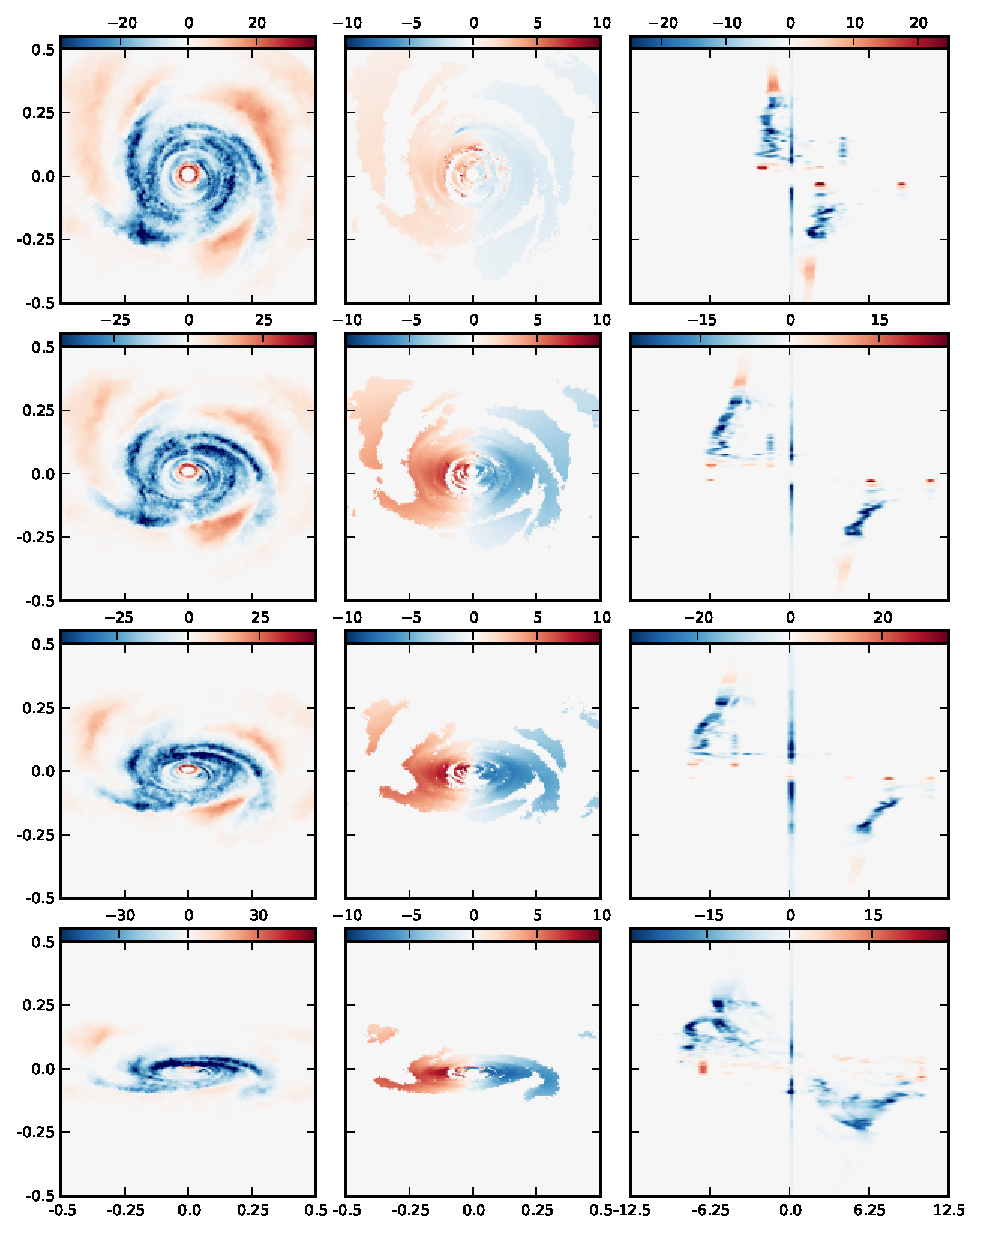
\includegraphics[width=164mm]{Figures/sim/appendix_inclinations2.eps}

 \caption{C$^{17}$O 3$\rightarrow$2 {\bf left:} Continuum subtracted integrated intensity map (in K$\,$km$\,$s$^{-1}$). {\bf Centre:} Intensity weighted velocity map (in km$\,$s$^{-1}$). {\bf Right:} Position-velocity diagram with intensities in K. The inclinations shown from top to bottom are 75$^\circ$, 45$^\circ$, 30$^\circ$ and 15$^\circ$ to edge on.}
\end{figure*}

%\begin{figure*}
% 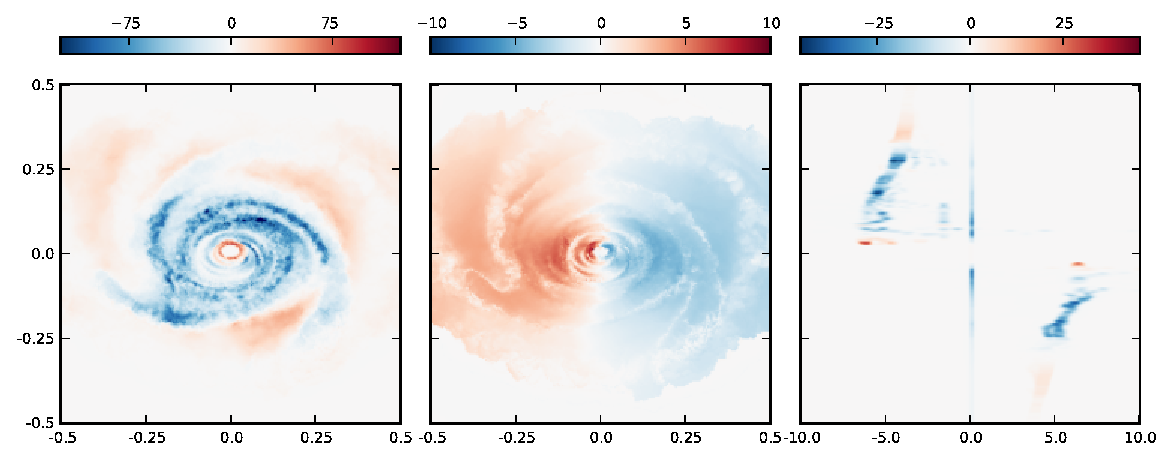
\includegraphics[width=164mm]{Figures/sim/imageC17O_3-2_45deg_all.eps}
%
% \caption{C$^{17}$O 3$\rightarrow$2 inclined at 45$^\circ$ to edge on. The three panels are: %{\bf left:} Continuum subtracted integrated intensity map (in K$\,$km$\,$s$^{-1}$). {\bf %Centre:} Intensity weighted velocity map (in km$\,$s$^{-1}$). {\bf Right:} Position-velocity %diagram with intensities in K.}
%\end{figure*}
%
%\begin{figure*}
% 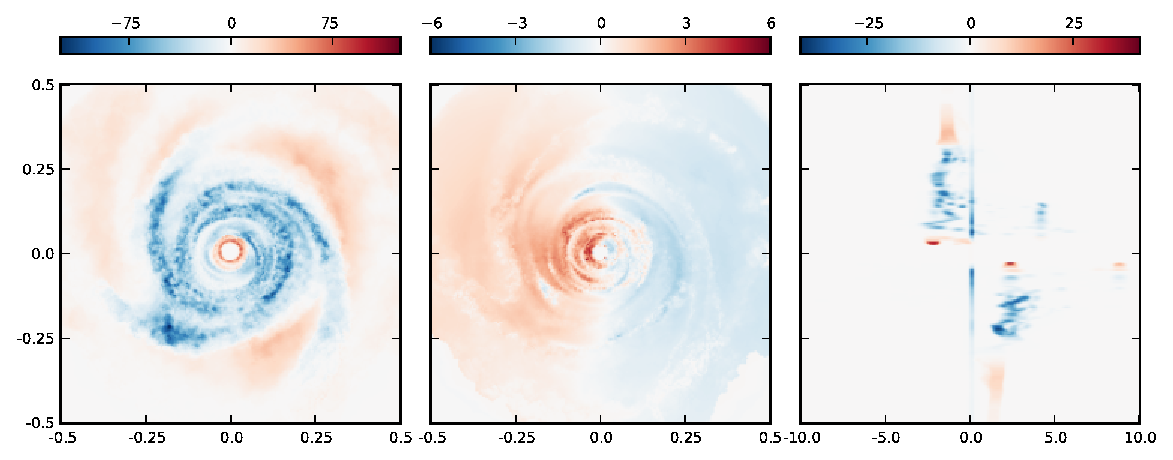
\includegraphics[width=164mm]{Figures/sim/imageC17O_3-2_75deg_all.eps}
%
% \caption{C$^{17}$O 3$\rightarrow$2 inclined at 75$^\circ$ to edge on. The three panels are: %{\bf left:} Continuum subtracted integrated intensity map (in K$\,$km$\,$s$^{-1}$). {\bf %Centre:} Intensity weighted velocity map (in km$\,$s$^{-1}$). {\bf Right:} Position-velocity %diagram with intensities in K.}
%\end{figure*}

%\begin{figure}
% 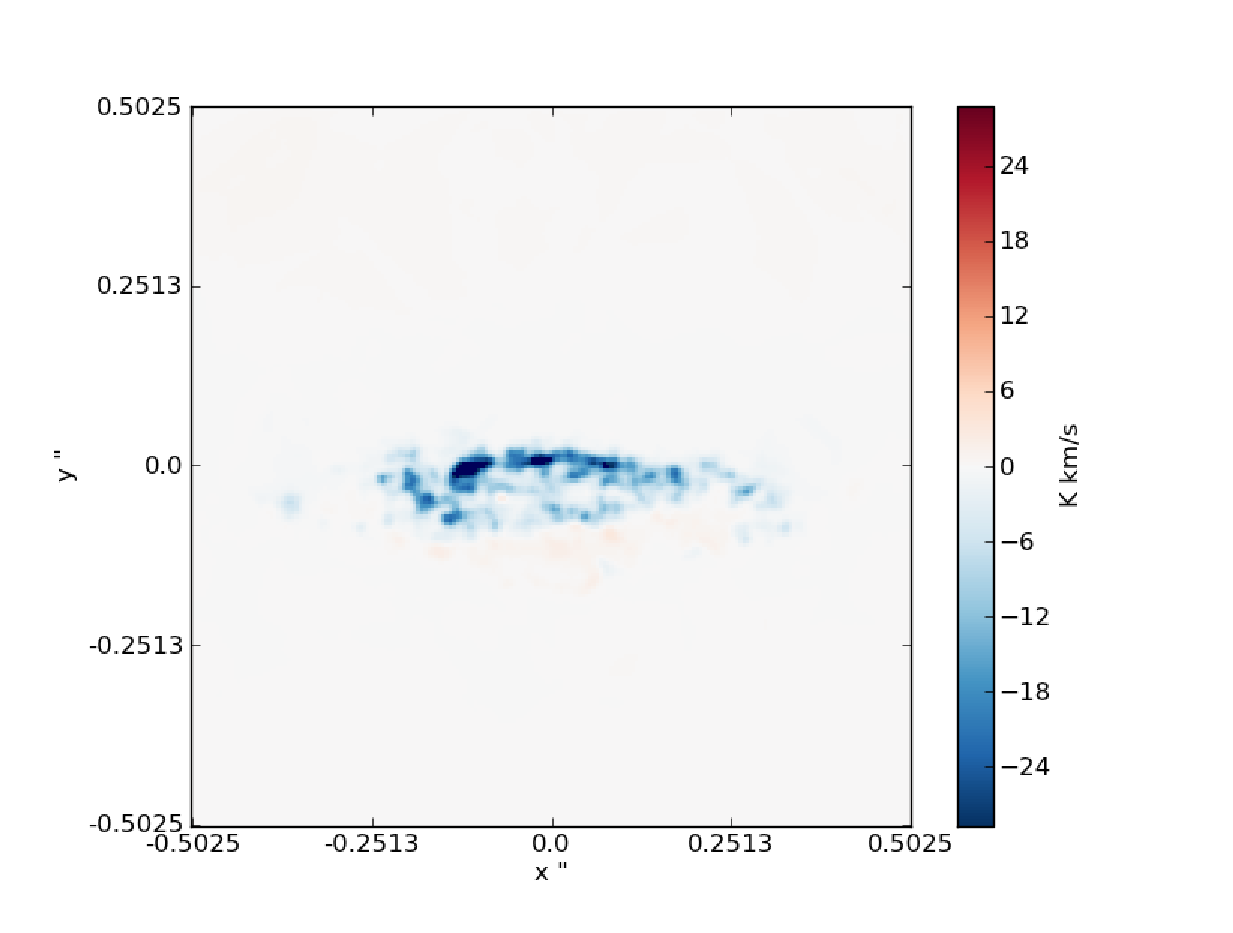
\includegraphics[width=84mm]{Figures/sim/imageC18O_3-2_15deg_contSub.eps}
%
% \caption{C18O 3-2 15 deg Continuum subtracted mom0}
%\end{figure}
%
%%\begin{figure}
%% 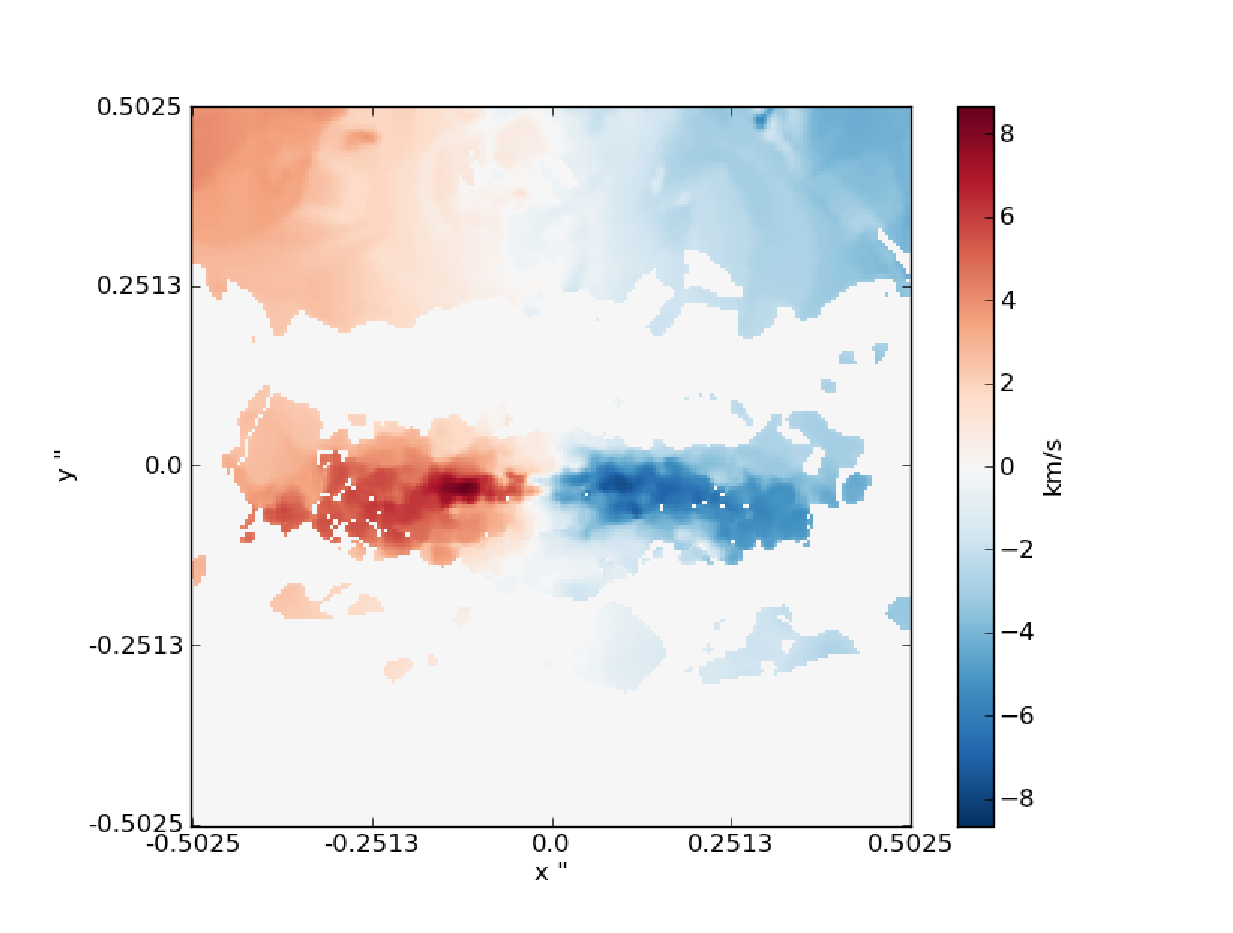
\includegraphics[width=84mm]{Figures/sim/imageC18O_3-2_15deg_mom1.eps}
%%
%% \caption{C18O 3-2 15 deg mom1map}
%%\end{figure}
%
%\begin{figure}
% 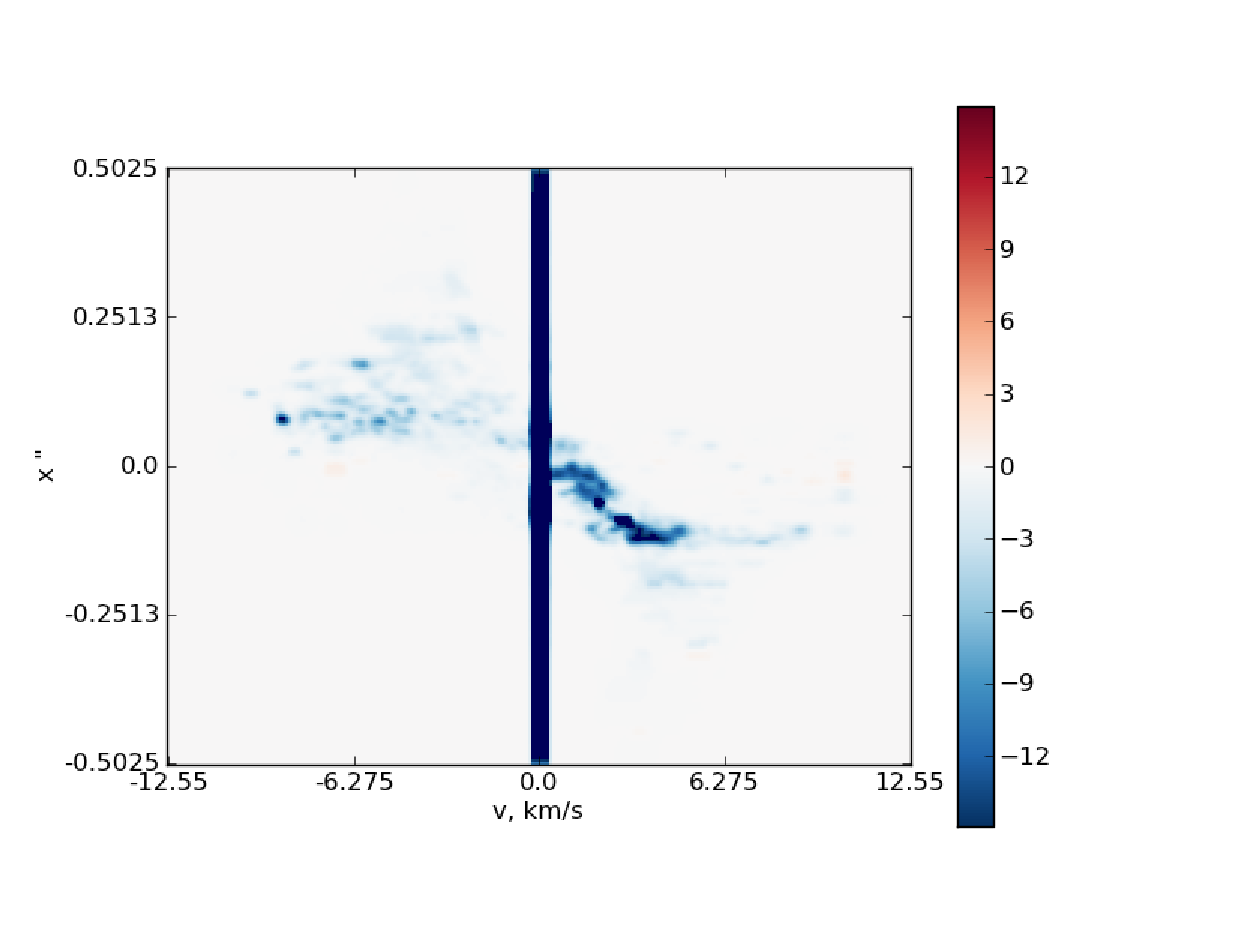
\includegraphics[width=84mm]{Figures/sim/imageC18O_3-2_15deg_PV_centre.eps}
%
% \caption{C18O 3-2 PV 15 deg through centre}
%\end{figure}
%
%
%\begin{figure}
% 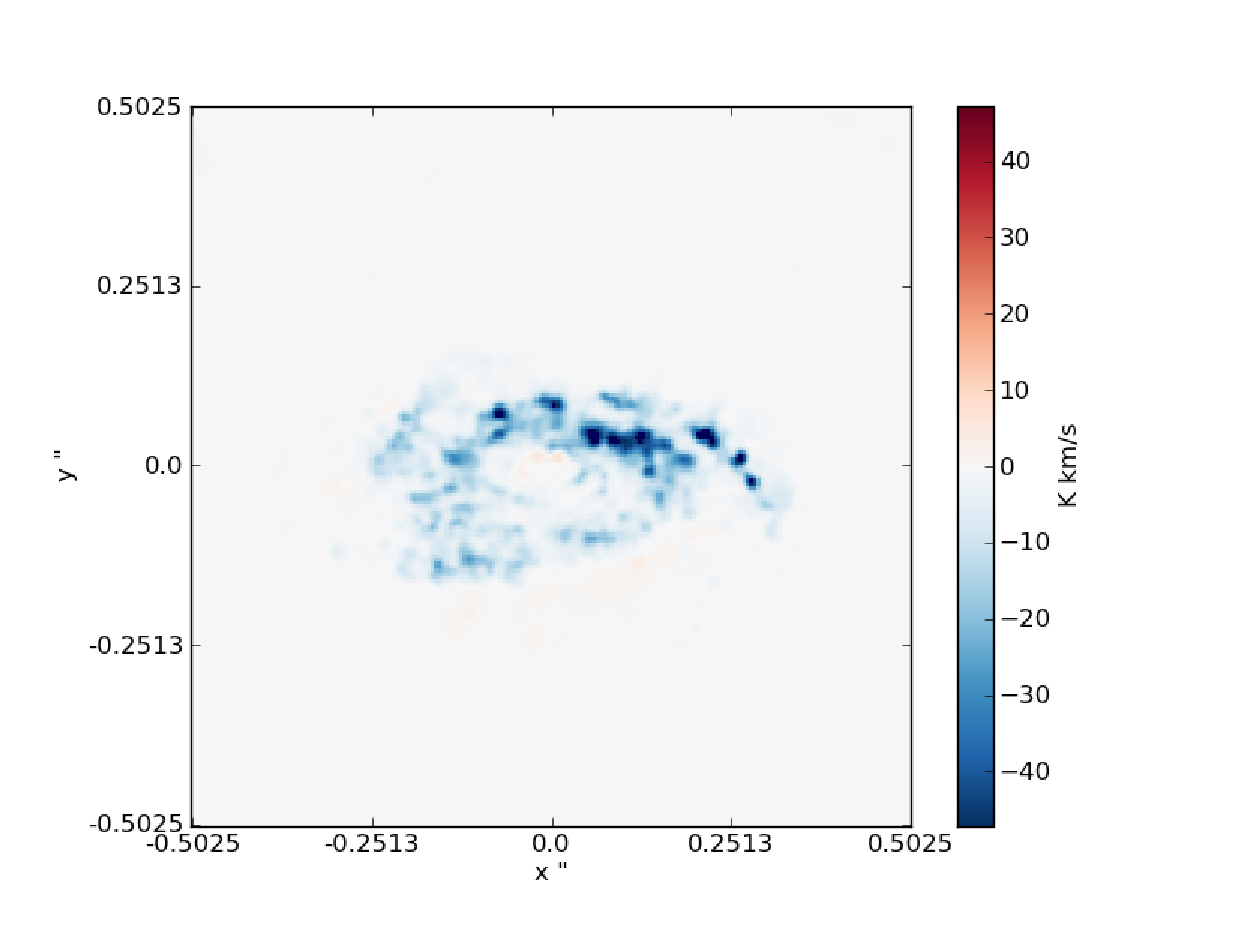
\includegraphics[width=84mm]{Figures/sim/imageC18O_3-2_30deg_contSub.eps}
%
% \caption{C18O 3-2  30 deg Continuum subtracted mom0}
%\end{figure}


%\begin{figure}
% 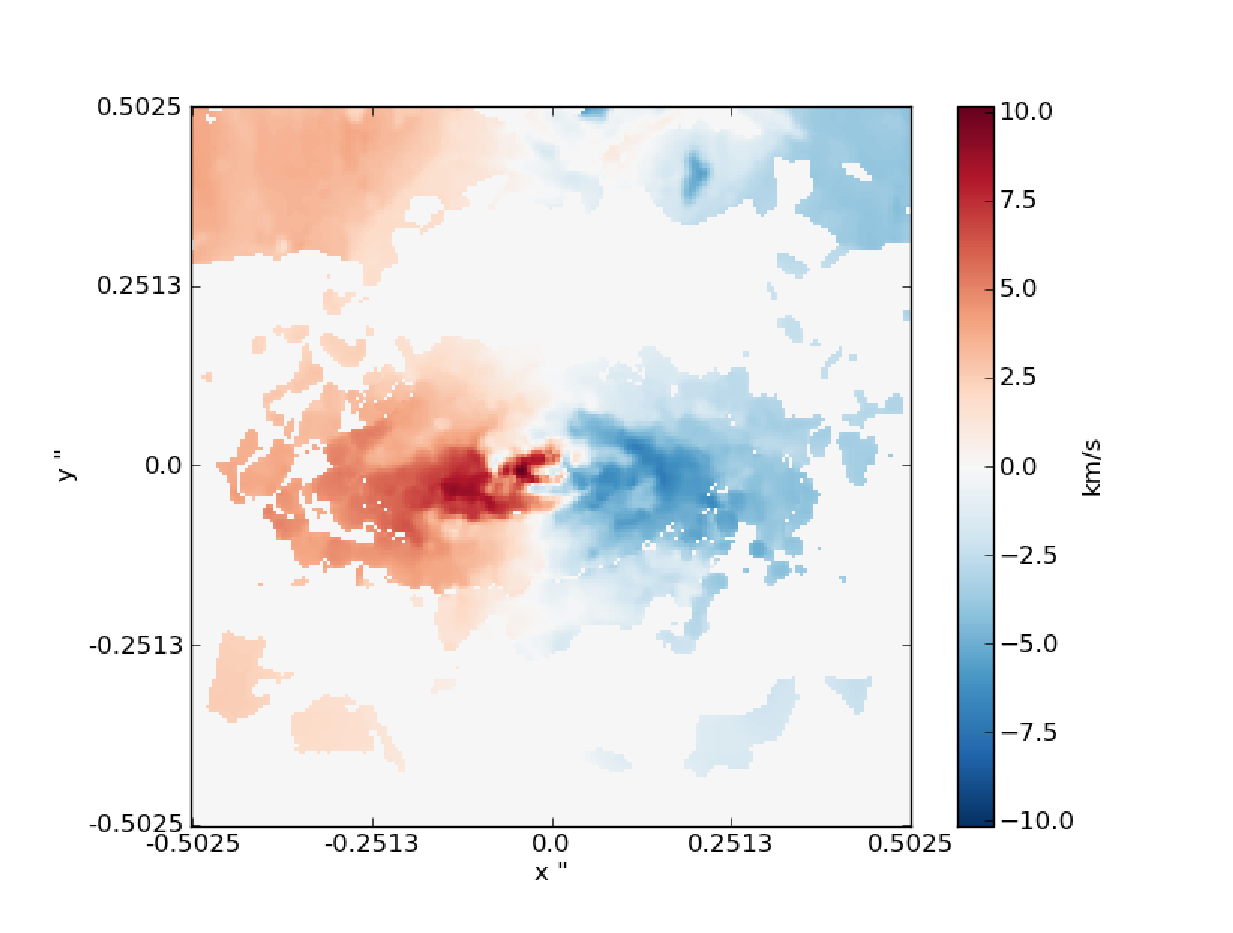
\includegraphics[width=84mm]{Figures/sim/imageC18O_3-2_30deg_mom1.eps}
%
% \caption{C18O 3-2 30 deg mom1map}
%\end{figure}

%\begin{figure}
% 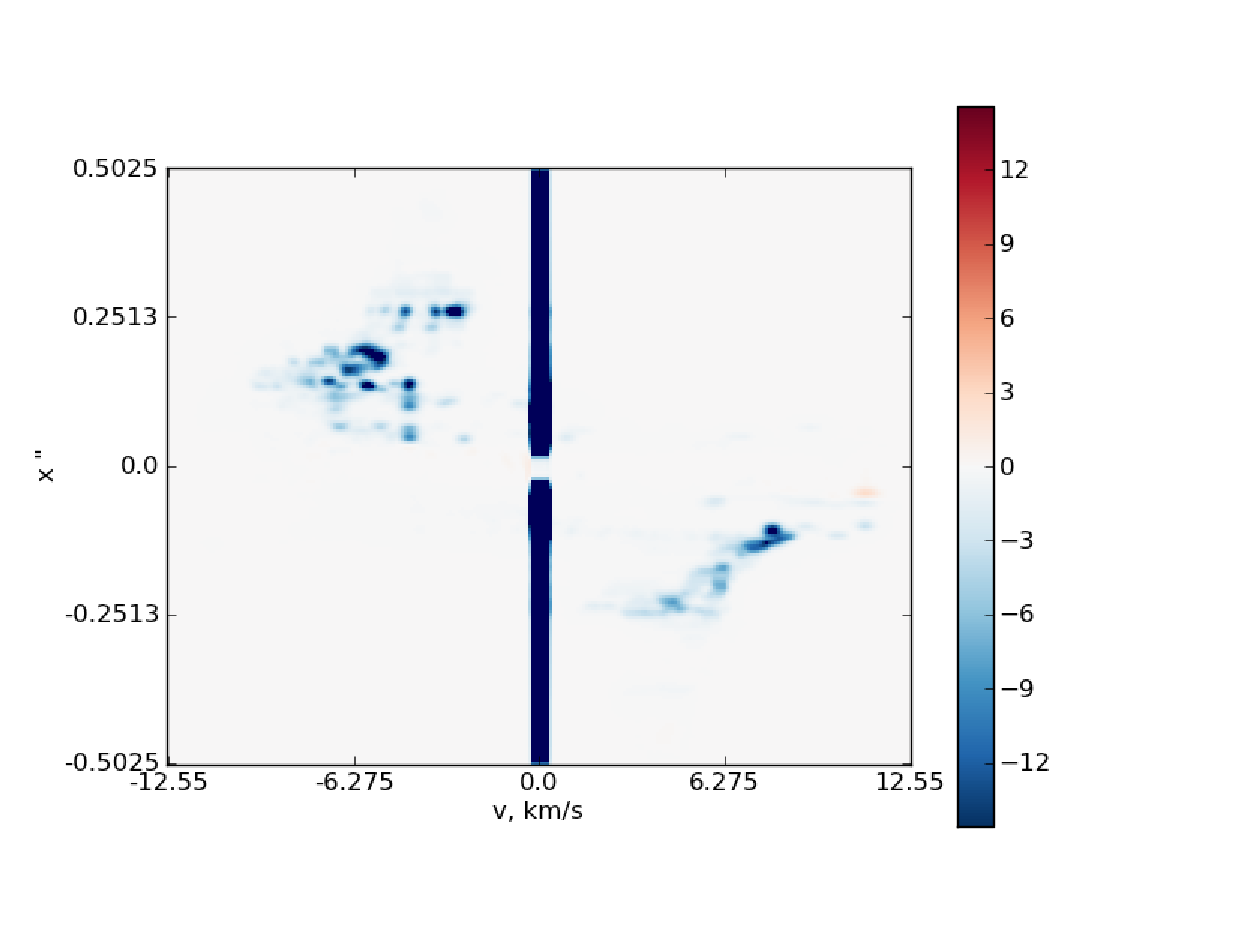
\includegraphics[width=84mm]{Figures/sim/imageC18O_3-2_30deg_PV_centre.eps}
%
% \caption{C18O 3-2 30 deg PV through centre}
%\end{figure}
%
%\begin{figure}
% 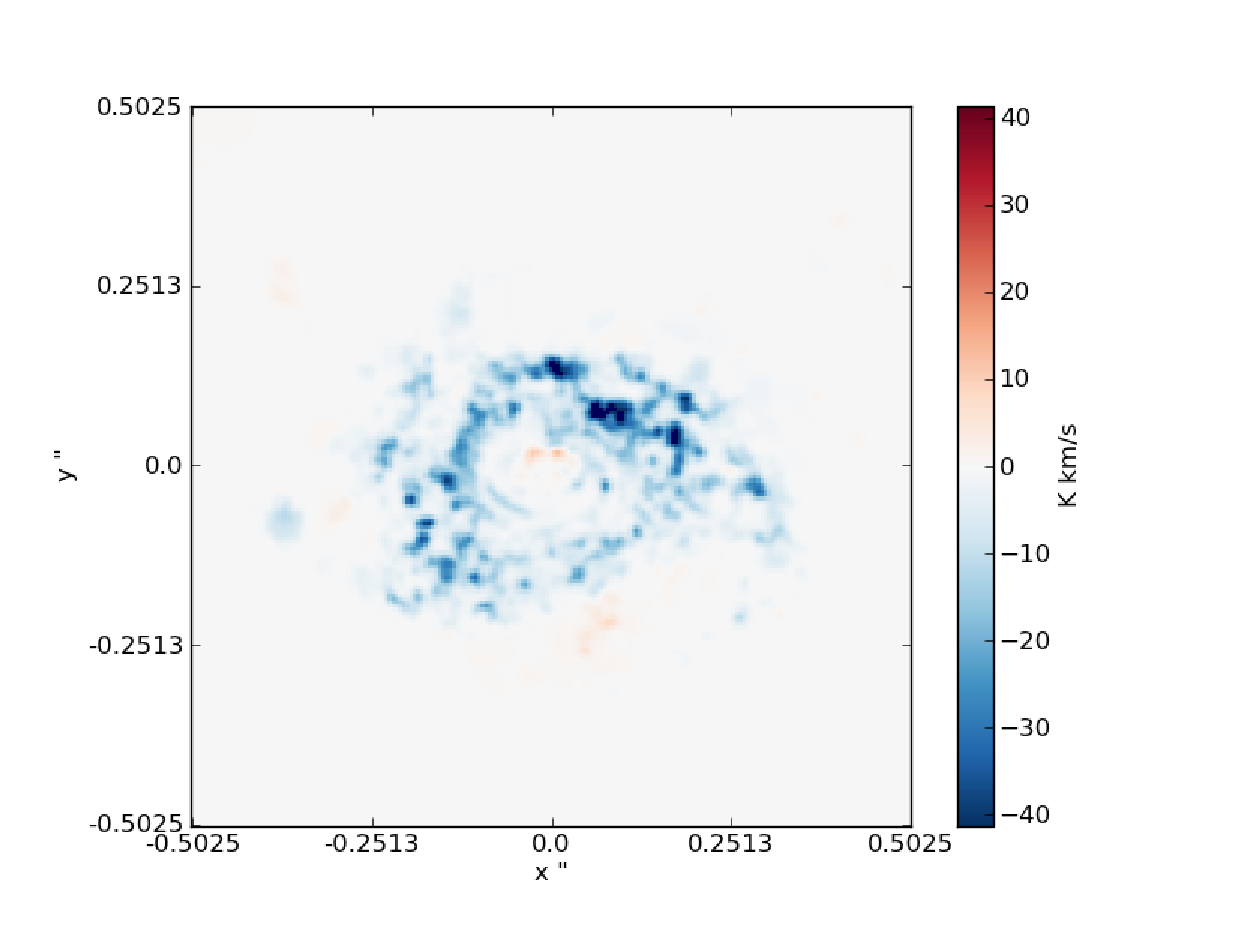
\includegraphics[width=84mm]{Figures/sim/imageC18O_3-2_45deg_contSub.eps}
%
% \caption{C18O 3-2 45 deg Continuum subtracted mom0}
%\end{figure}
%
%%\begin{figure}
%% 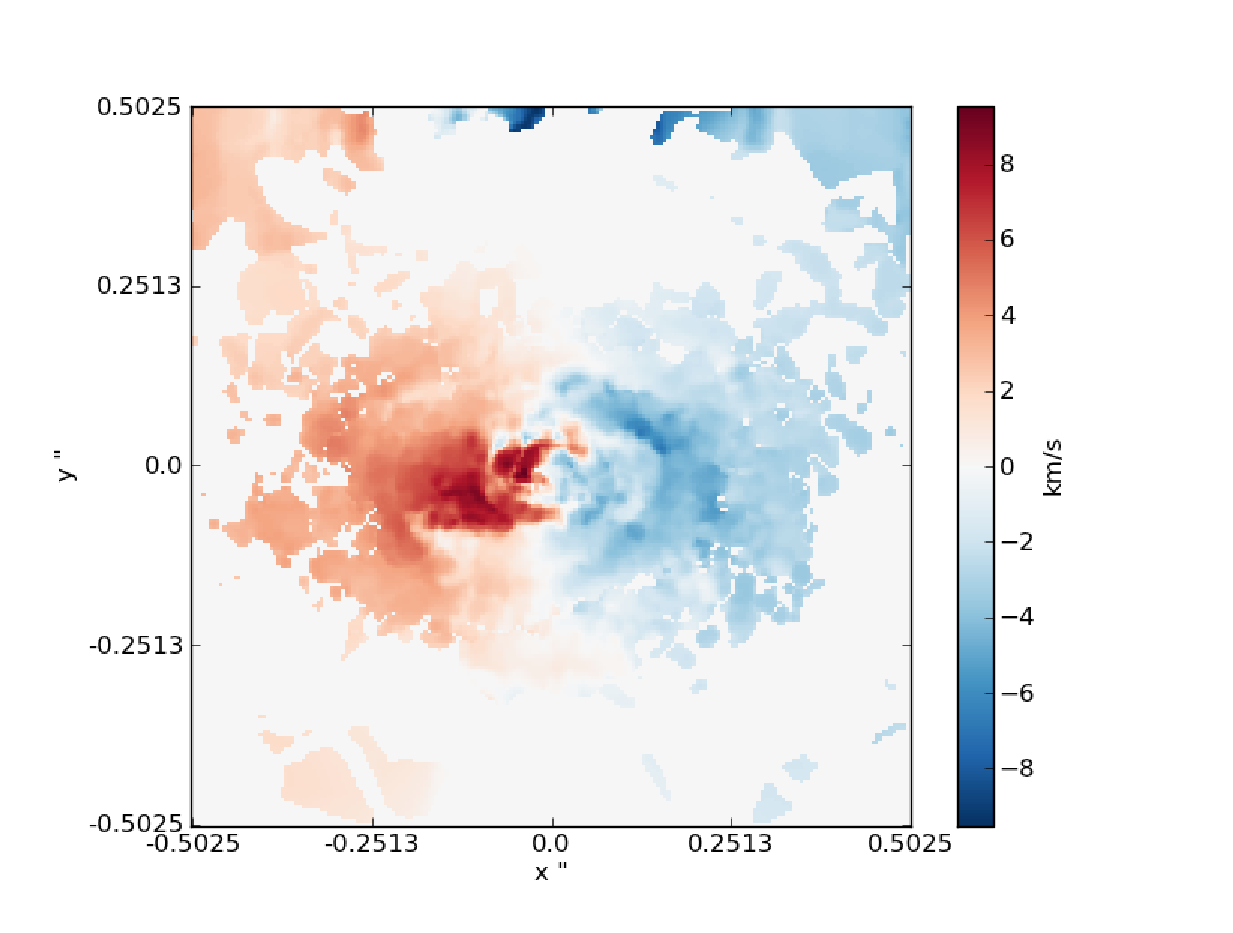
\includegraphics[width=84mm]{Figures/sim/imageC18O_3-2_45deg_mom1.eps}
%%
%% \caption{C18O 3-2 45 deg mom1map}
%%\end{figure}
%
%\begin{figure}
% 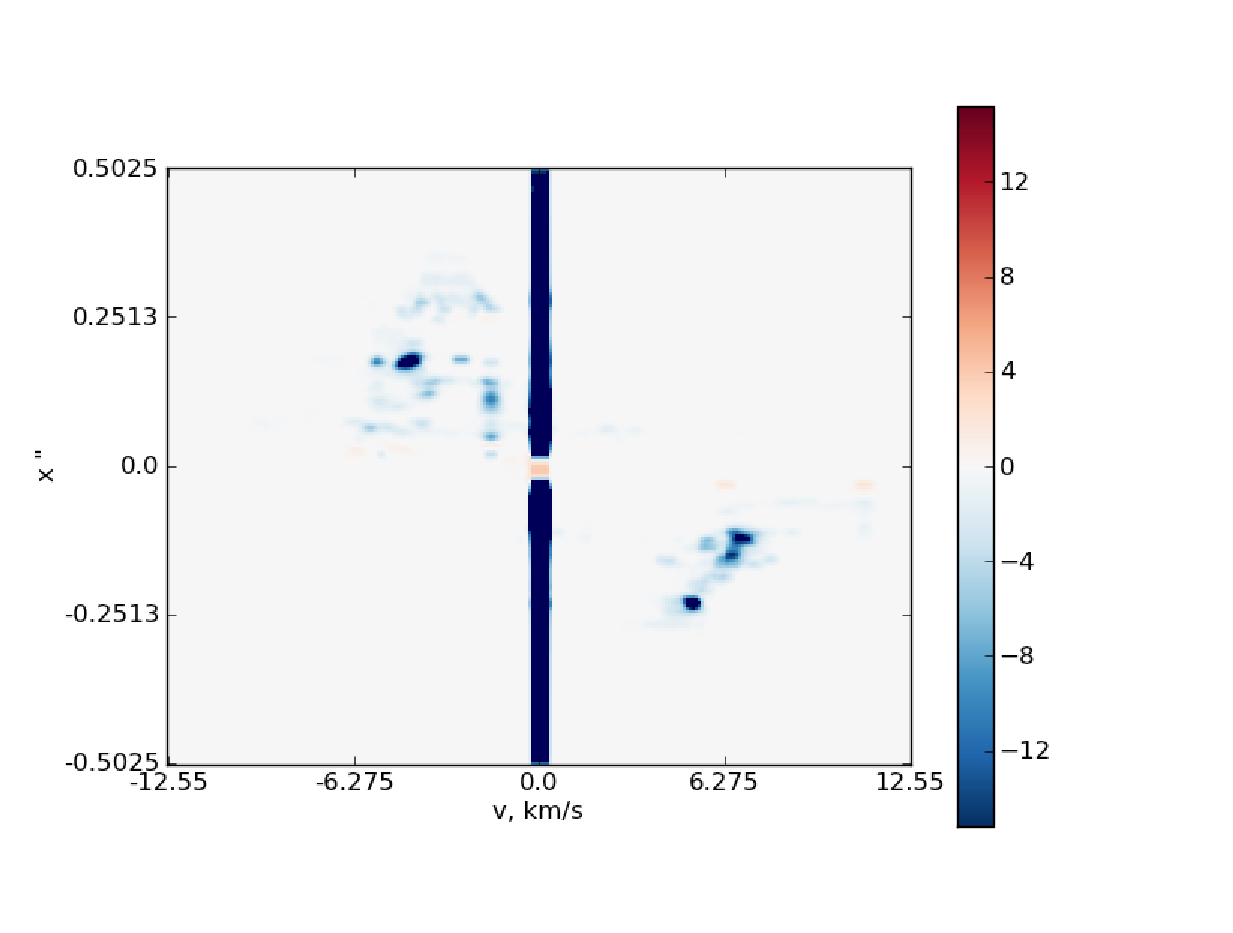
\includegraphics[width=84mm]{Figures/sim/imageC18O_3-2_45deg_PV_centre.eps}
%
% \caption{C18O 3-2 45 deg PV through centre}
%\end{figure}
%
%
%\begin{figure}
% 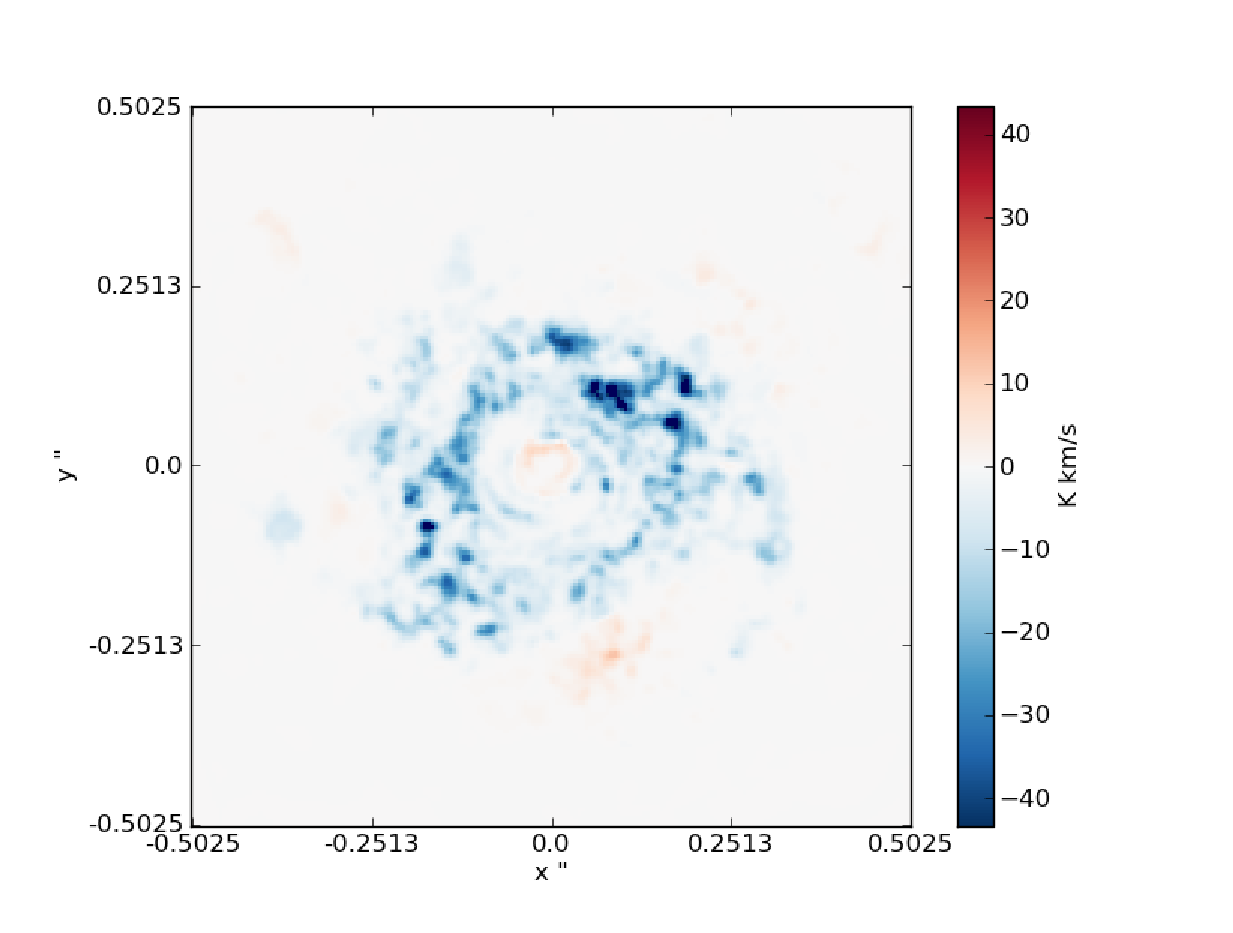
\includegraphics[width=84mm]{Figures/sim/imageC18O_3-2_60deg_contSub.eps}
%
% \caption{C18O 3-2 60 deg Continuum subtracted mom0}
%\end{figure}
%
%%\begin{figure}
%% 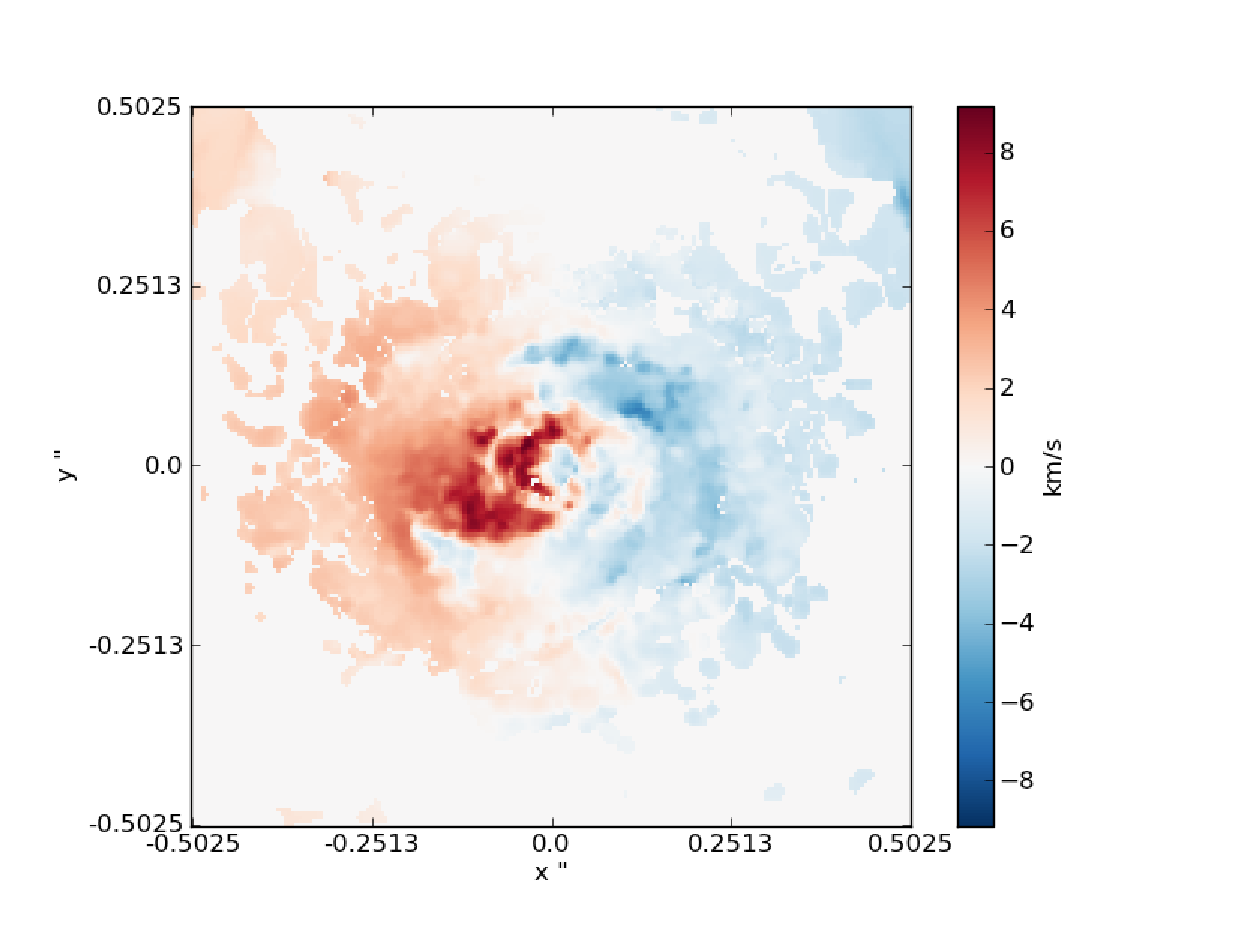
\includegraphics[width=84mm]{Figures/sim/imageC18O_3-2_60deg_mom1.eps}
%%
%% \caption{C18O 3-2 60 deg mom1map}
%%\end{figure}
%
%\begin{figure}
% 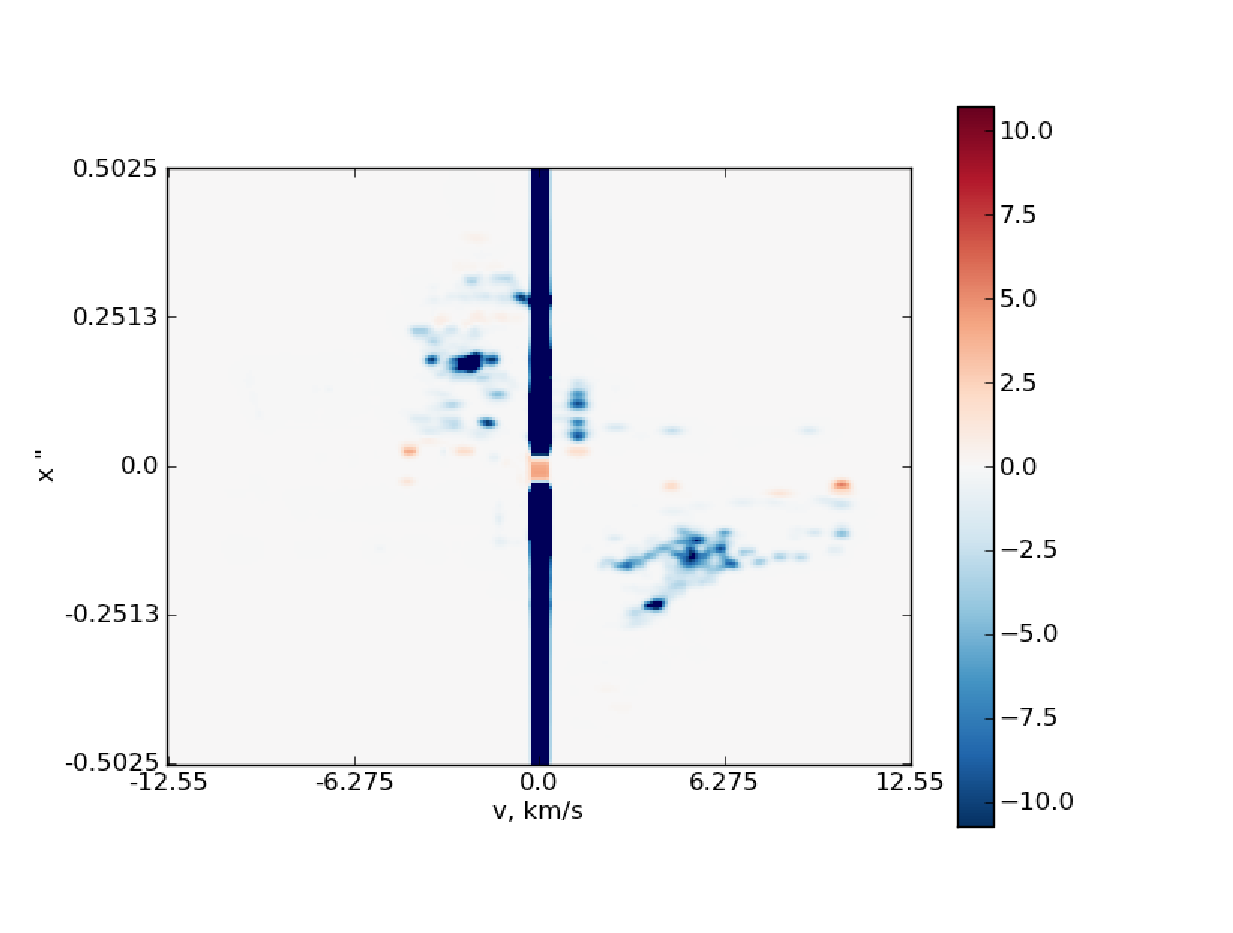
\includegraphics[width=84mm]{Figures/sim/imageC18O_3-2_60deg_PV_centre.eps}
%
% \caption{C18O 3-2 60 deg PV through centre}
%\end{figure}
%
%\begin{figure}
% 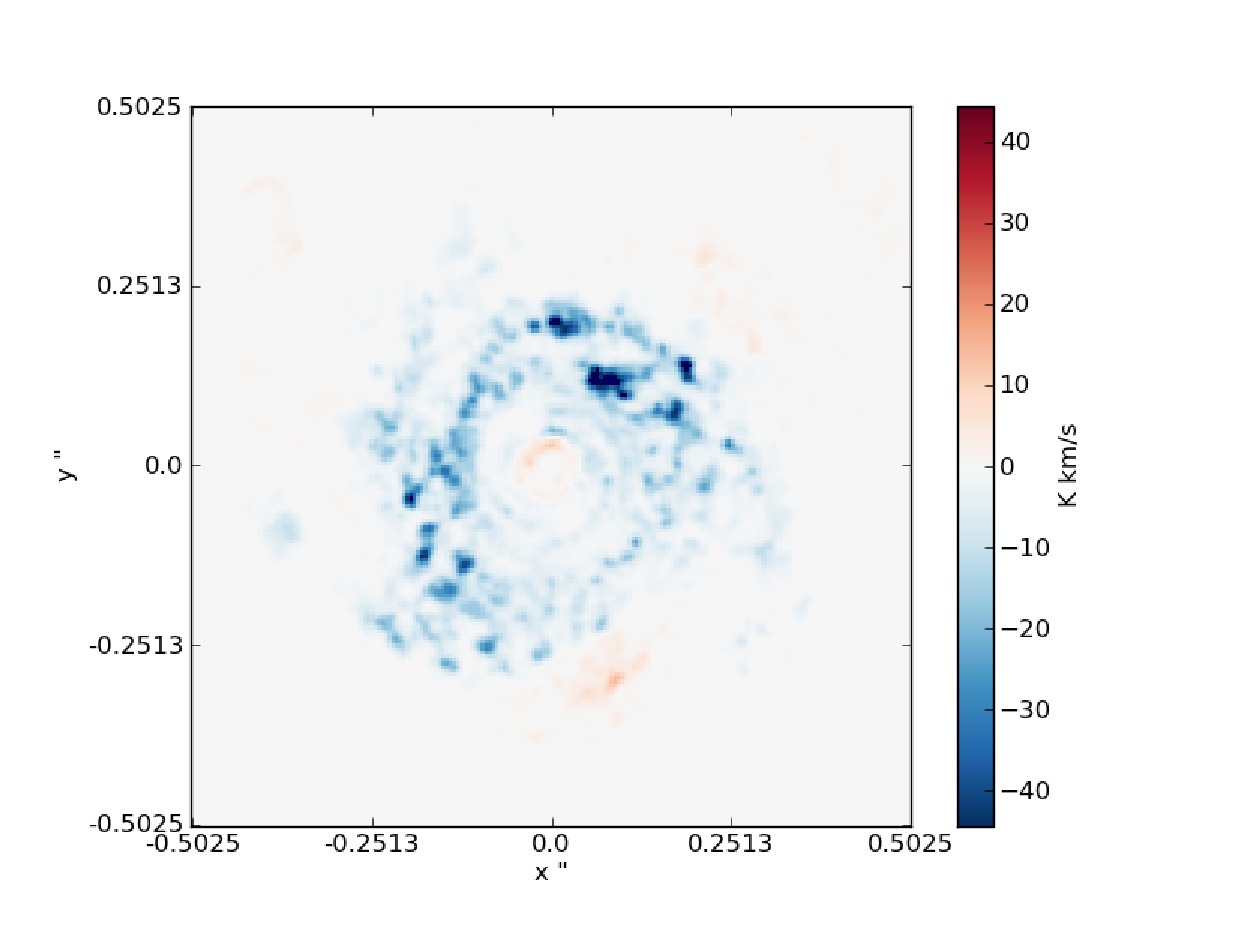
\includegraphics[width=84mm]{Figures/sim/imageC18O_3-2_75deg_contSub.eps}
%
% \caption{C18O 3-2 75 deg Continuum subtracted mom0}
%\end{figure}
%
%%\begin{figure}
%% 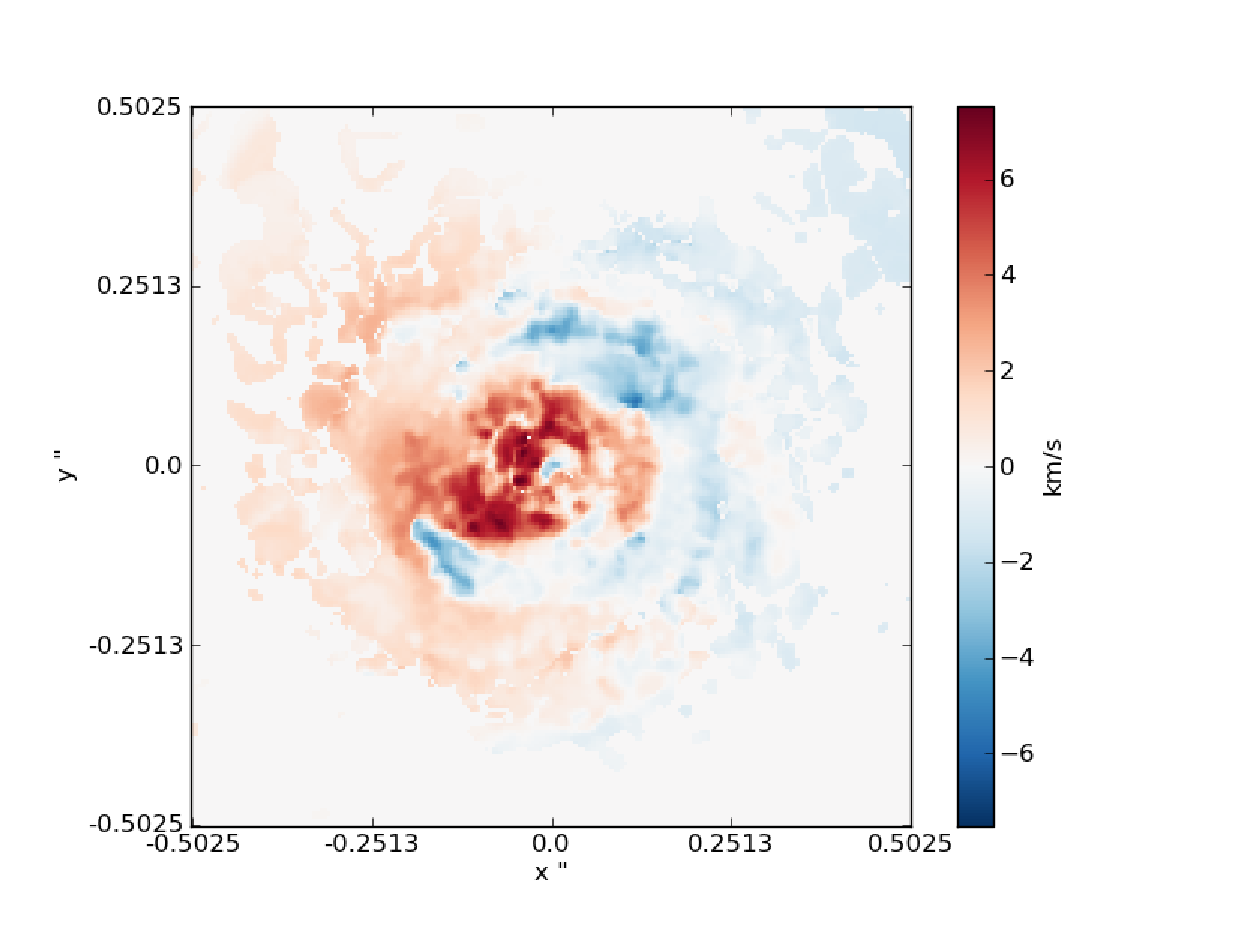
\includegraphics[width=84mm]{Figures/sim/imageC18O_3-2_75deg_mom1.eps}
%%
%% \caption{C18O 3-2 75 deg mom1map}
%%\end{figure}
%
%\begin{figure}
%%  \showthe\columnwidth % Use this to determine the width of the figure.
%  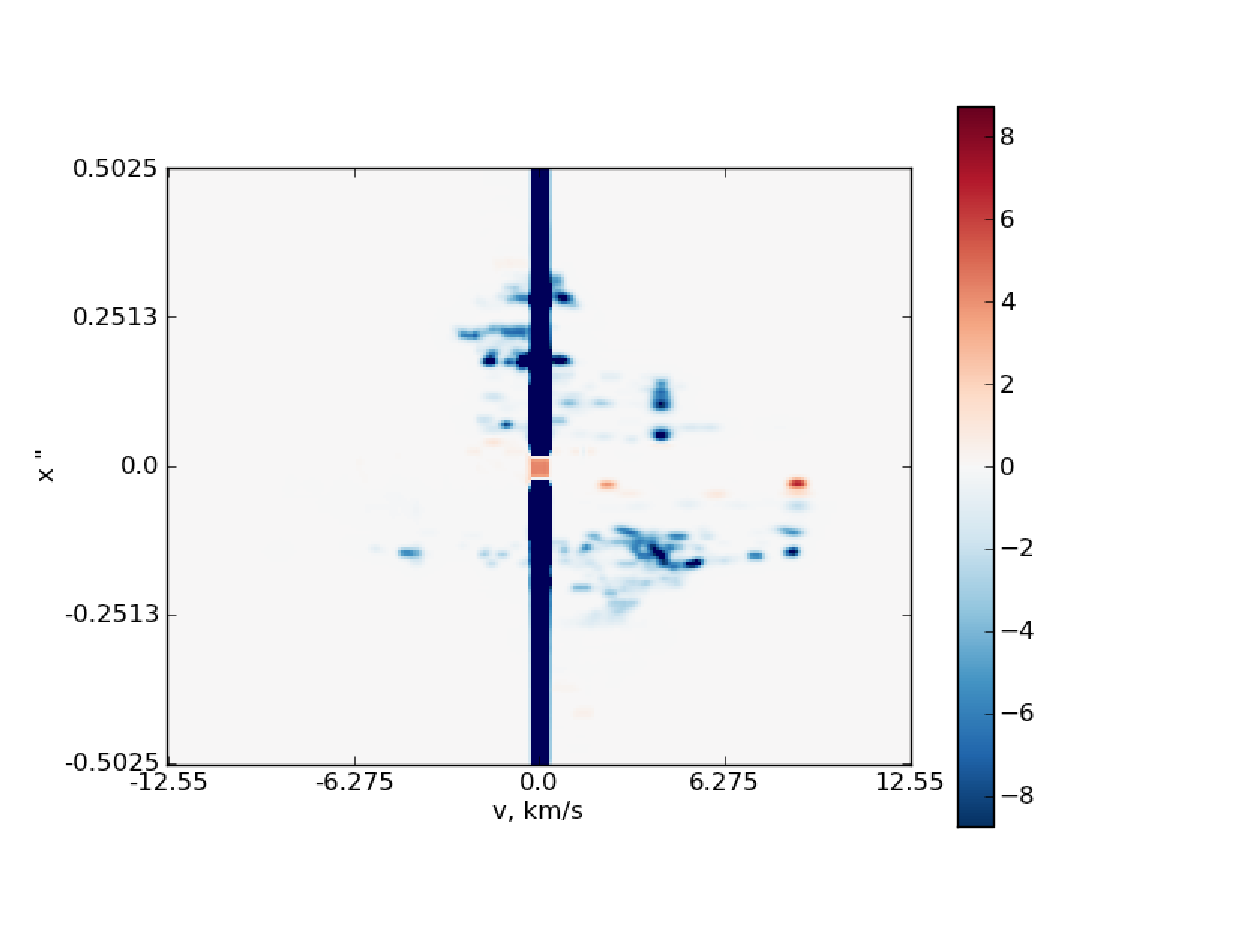
\includegraphics[width=84mm]{Figures/sim/imageC18O_3-2_75deg_PV_centre.eps}
%  \caption{C18O 3-2 75 deg PV through centre}
%\end{figure}

\bsp
%
\label{lastpage}
%
\end{document}
